\documentclass[12pt, a4paper]{article}

% Packages essentiels
\usepackage[utf8]{inputenc}
\usepackage[T1]{fontenc}
\usepackage[french]{babel}
\usepackage{parskip}
\usepackage{mathptmx} % Times New Roman
\usepackage{amsmath}
\usepackage{enumitem}
\usepackage{setspace}
\usepackage{fancyhdr}
\usepackage{titlesec}
\usepackage{pdfpages}
\usepackage{graphicx}
\usepackage{float}
\usepackage{longtable}
\usepackage{makecell}

%highlight
\usepackage{soul}
\usepackage{xcolor}

%%%%%%%%%%%%%%%%%%%%%%%%%%%%%%%%%%%%%%%%%%%%%%%%%%%%%%%%%%%%%%%%%%%%%%%%%%%%%%%%%%%%%%%%%%
\usepackage{csquotes}
\usepackage{xurl}
\usepackage{hyperref}%[hidelinks]
\usepackage{apacite}

%%%%%%%%%%%%%%%%%%%%%%%%%%%%%%%%%%%%%%%%%%%%%%%%%%%%%%%%%%%%%%%%%%%%%%%%%%%%%%%%%%%%%%%%%%

% Marges : 2.5 cm gauche/droite, 3 cm haut/bas (avec pagination)
\usepackage[left=2.5cm, right=2.5cm, top=3cm, bottom=3cm]{geometry}

% Interligne 1.5
\onehalfspacing

% Correction headheight pour fancyhdr
\setlength{\headheight}{14.5pt}
\addtolength{\topmargin}{-2.5pt}

% Configuration de l'en-tête et pagination
\pagestyle{fancy}
\fancyhf{}
\fancyhead[R]{\thepage.}
\renewcommand{\headrulewidth}{0pt}
\renewcommand{\footrulewidth}{0pt}

% Subsubsection (alinéas) : italique
%\titleformat{\subsubsection}
%  {\normalfont\normalsize\itshape}{\thesubsubsection}{1em}{}

\begin{document}

% Page de garde
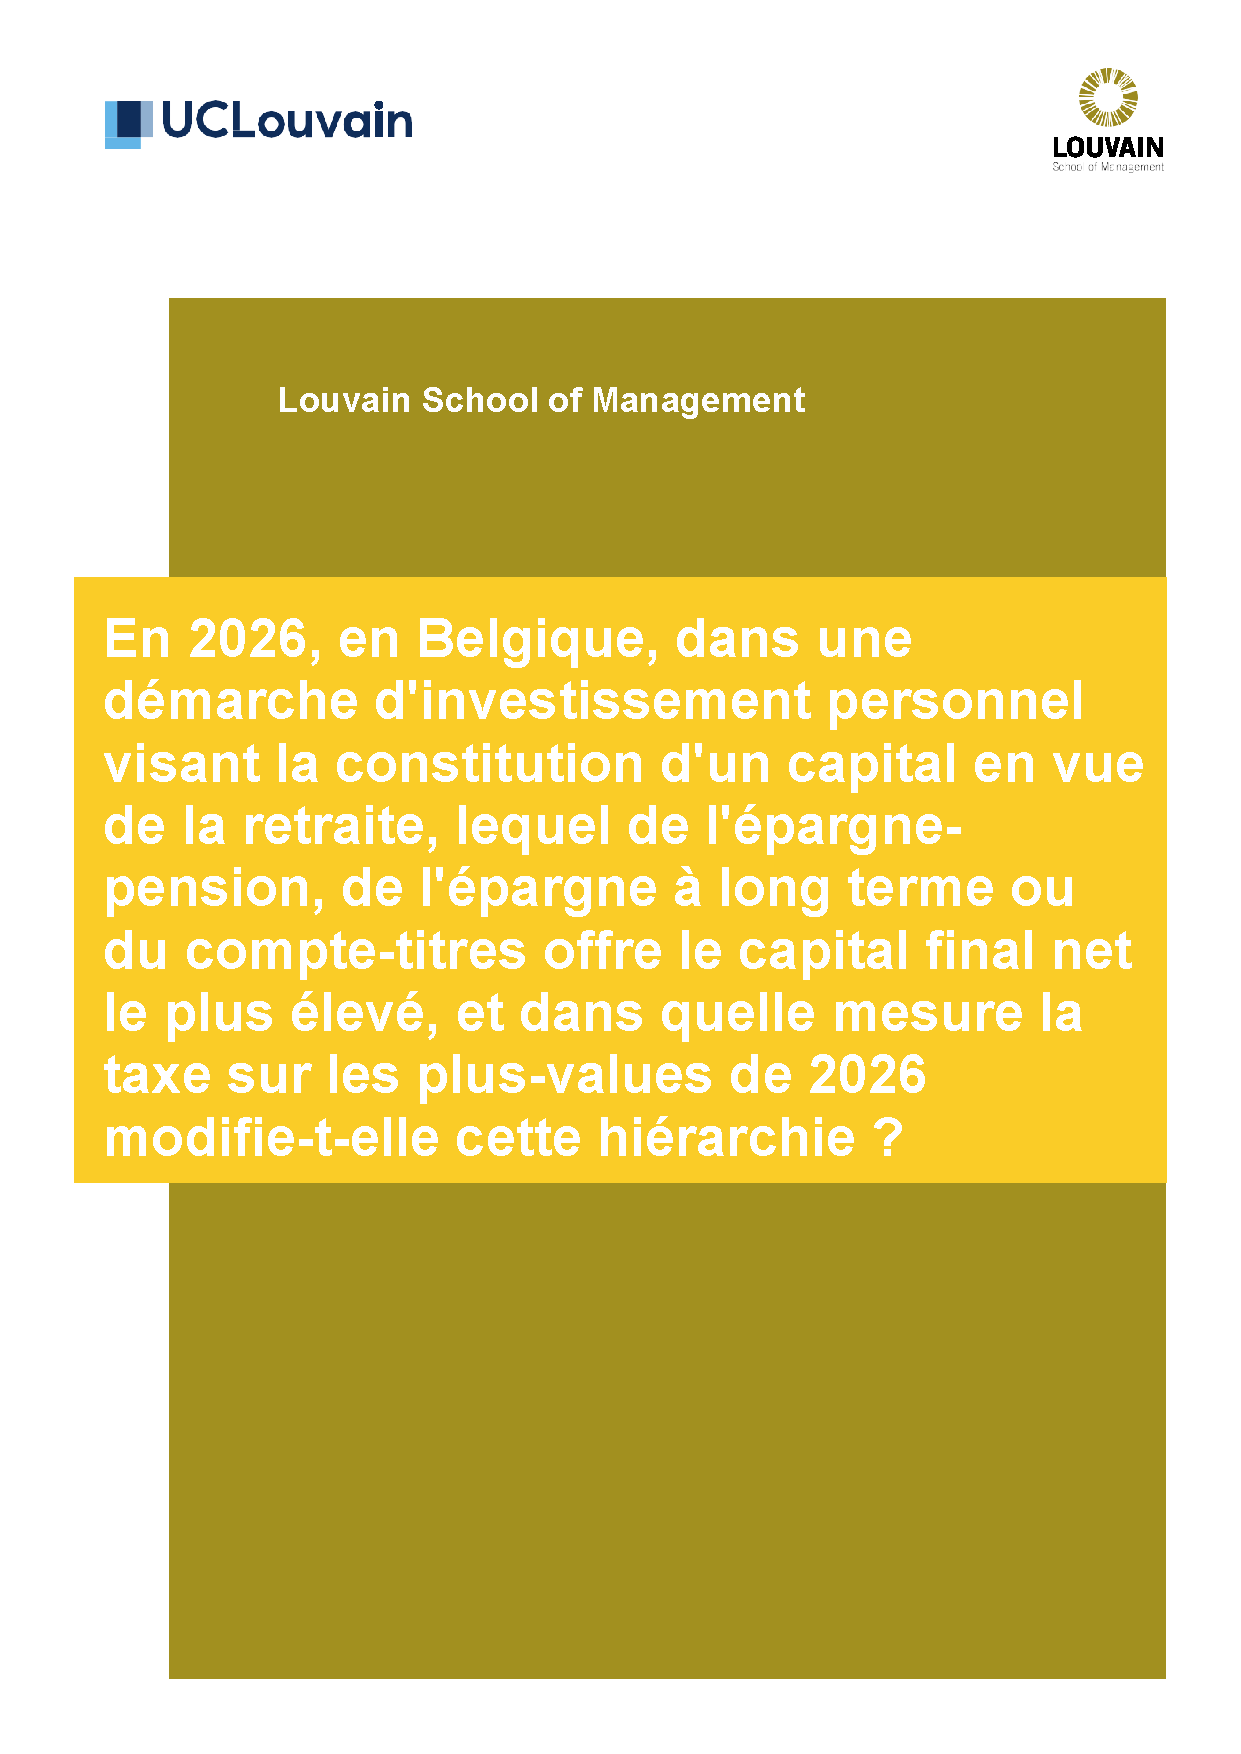
\includepdf[pages=-]{media/front.pdf}

\newpage
\pagestyle{empty}

\section*{Avant-propos}
\addcontentsline{toc}{section}{Avant-propos}

Ce travail est né d'un intérêt personnel pour l'investissement. Depuis quelques années,
j'investis en ETF et j'ai consommé beaucoup de contenu portant sur l'investissement
passif à long terme en fonds indiciels. Des créateurs comme
\href{https://www.youtube.com/@gregoryguilmin}{Gregory Guilmin} ou
\href{https://www.youtube.com/@matthiasbaccino}{Matthias Baccino} (ce dernier
étant le fondateur de Trade Republic, un néocourtier proposant un accès simplifié aux
marchés financiers à frais réduits) contribuent à populariser cette
approche. Ils défendent l'investissement en ETF passifs sur le long terme comme étant la
meilleure façon d'investir, supérieure à d'autres approches parmi lesquelles
figurent notamment les produits d'assurance-vie. J'ai toutefois remarqué que ces
comparaisons sont souvent menées avec des rendements différents selon les véhicules,
le taux le plus élevé étant systématiquement attribué au compte-titres et le plus
faible à l'assurance-vie. Il me semble que comparer des rendements inégaux ne permet
pas d'évaluer les véhicules en tant que tels ; une comparaison à rendement identique
serait bien plus éclairante. Gregory Guilmin, qui s'adresse
spécifiquement à un public belge, insiste par ailleurs sur le contexte fiscal
favorable dont bénéficiaient jusqu'à présent les investisseurs en Belgique, où les
plus-values boursières n'étaient pas taxées. Ce mouvement s'inscrit dans une
tendance plus large : les néocourtiers sont de plus en plus nombreux et rendent l'accès
aux marchés toujours plus accessible pour le grand public.

\hl{corriger et dire que c est cohérent de mettre un rendement identique
trop catégorique de dire que c était pas avantageux assurance vie,
c était juste mon hypothèse qu on va essayer de vérifier ici}

Par ailleurs, on a cherché à me proposer des produits d'assurance-vie de
branche~23 dans le cadre de l'épargne-pension et de l'épargne à long terme, auxquels
je n'ai pas souscrit. Pour évaluer leur pertinence dans ma situation, j'avais eu
recours à un simulateur en ligne permettant d'intégrer un montant investi (unique ou
périodique), les différents frais du produit et la durée de placement. J'avais ainsi
pu démontrer, dans mon cas précis, que ces produits ne s'avéraient pas avantageux.
Mais cette conclusion restait partielle. Je me suis toujours demandé si, quelle que soit
la configuration, il est réellement plus intéressant d'investir soi-même plutôt que de
recourir à ces enveloppes fiscales. J'ai toujours voulu réaliser ce genre de simulation
à plus grande échelle, en faisant varier les montants investis, les rendements et les
durées de placement. Ce travail de fin d'études m'en a fourni l'occasion, sous la
forme d'une simulation développée en Java, me permettant ainsi de combiner les
acquis de ce master en sciences de gestion avec mes compétences de développeur
professionnel.

\hl{pas citer java}

Je tiens à remercier [à compléter].

\newpage
\pagenumbering{Roman}
\pagestyle{fancy}
\tableofcontents

\newpage
\section*{Glossaire}
\addcontentsline{toc}{section}{Glossaire}

\begin{description}[leftmargin=4.5cm, style=sameline, font=\normalfont\bfseries]
  \item[OPCVM] \textit{Organisme de Placement Collectif en Valeurs Mobilières} — fonds d'investissement collectif permettant à des investisseurs de mettre en commun leurs ressources pour investir dans un portefeuille diversifié de titres financiers.

\end{description}
%https://fr.wikipedia.org/wiki/Organisme_de_placement_collectif_en_valeurs_mobili%C3%A8res
%https://fr.wikipedia.org/wiki/Organisme_de_placement_collectif_en_valeurs_mobili%C3%A8res
%https://fr.wikipedia.org/wiki/Fonds_n%C3%A9goci%C3%A9_en_bourse

\newpage
\pagenumbering{arabic}

\section{Contexte}

Au cours des dernières années, l'accès aux marchés financiers s'est profondément
démocratisé en Belgique. Le développement de néocourtiers à frais réduits et la
popularisation des fonds indiciels cotés (ETF) ont conduit un nombre croissant de
particuliers à gérer eux-mêmes leurs investissements, en dehors de tout cadre
institutionnel. Dans les débats publics sur l'investissement individuel, cette
approche est fréquemment mise en regard des enveloppes fiscales dédiées à la
constitution d'un capital pour la retraite que constituent l'épargne-pension et
l'épargne à long terme. La question de savoir laquelle de ces stratégies est la plus
avantageuse financièrement est régulièrement soulevée, sans toujours faire l'objet
d'une analyse rigoureuse à hypothèses comparables.

\subsection{Régime fiscal avant 2026}

Jusqu'au 31~décembre~2025, la Belgique se distinguait par l'absence de taxation des
plus-values réalisées par les particuliers dans le cadre de la gestion normale de
leur patrimoine privé \cite[art.~90]{cir92_2025}. Seules les opérations à caractère
spéculatif faisaient l'objet d'une imposition, au taux de 33\,\%
\cite[art.~171]{cir92_2025}. Ce régime conférait à l'investissement direct en
compte-titres un avantage structurel significatif, la totalité des gains en capital
accumulés sur le long terme lui demeurant intégralement acquise.

En parallèle, l'épargne-pension et celle à long terme prennent la forme de
contrats d'assurance-vie par lesquels le preneur verse des primes et reçoit
un capital à l'échéance fixée si l'assuré est en vie. Les primes versées bénéficient,
sous certaines conditions, d'une réduction d'impôt \cite[p.~115-116]{Binon2016},
mais ces enveloppes imposent en contrepartie une taxation à la sortie ainsi qu'une
éventuelle taxe à l'entrée. La comparaison entre les deux
approches constituait donc déjà, dans ce cadre, une question pertinente.

\subsection{Régime fiscal de 2026}

À compter du 1\textsuperscript{er}~janvier~2026, ce paysage a été profondément
modifié. Le projet de loi du 17~décembre~2025 introduit un impôt sur les plus-values des
actifs financiers réalisées en dehors de toute activité professionnelle, au taux de
10\,\%, après exonération d'une première tranche annuelle de 10\,000~euros
\cite[p.~4-5, 9]{chambre2025pv_actifs}. Les actifs relevant de l'épargne-pension et
de l'épargne à long terme sont explicitement exclus du champ de cet impôt
\cite[p.~39]{chambre2025pv_actifs}.

Cette réforme modifie structurellement les termes de la comparaison entre
investissement direct et enveloppes fiscales. Elle réduit la rentabilité nette du
compte-titres tout en laissant inchangée celle des contrats d'assurance-vie dédiés à
l'épargne retraite, créant ainsi une asymétrie nouvelle qui justifie une réévaluation
de la hiérarchie entre ces véhicules.

Les chapitres suivants définissent précisément chacun de ces véhicules, en détaillant
leur fonctionnement, leur structure de coûts et leur régime fiscal, afin de poser les
bases nécessaires à la simulation comparative.

\newpage
\section{Cadre de travail}

\subsection{Délimitation du périmètre de l'étude}

Afin de maintenir la rigueur et la comparabilité des analyses, l'étude s'inscrit dans
un cadre délibérément circonscrit, dont les limites sont les suivantes.

\textbf{Nature de l'investisseur.} L'analyse porte exclusivement sur un particulier
qui gère son épargne à titre personnel, de sa propre initiative. Les mécanismes
collectifs d'épargne-pension organisés dans le cadre de l'emploi, à savoir les
fonds de pension d'entreprise et les engagements individuels de pension, sont exclus du
champ de l'étude. \hl{+ profil des risques, personne qui investissent 100 pc en action
car accumulant c est la tendance plus pas plus value obligataire}

\textbf{Véhicule de placement retenu pour le compte-titres.} Conformément à la
tendance actuelle, la comparaison porte sur des comptes-titres ouverts auprès de
néobrokers à bas frais. Ce choix se justifie par le fait que c'est précisément ce
type de plateforme qui est le plus mis en avant dans les débats publics sur
l'investissement individuel, et que la structure de coûts qui lui est associée est
significativement différente de celle des banques traditionnelles. 

\textbf{Horizon d'investissement.} L'horizon de référence est fixé à 65~ans pour
l'ensemble des comparaisons. Bien que l'âge légal de la retraite évolue progressivement
vers 67~ans et que le compte-titres ou l'épargne à long terme n'imposent pas de borne
supérieure stricte, retenir 65~ans comme horizon commun garantit une homogénéité
totale entre tous les véhicules analysés et correspond à l'âge pivot utilisé par la
législation relative à l'épargne-pension. L'effort d'épargne s'arrête donc à cet âge,
l'objectif étant de permettre à l'investisseur de profiter de son capital constitué.

\textbf{Mode de sortie du capital.} L'étude considère exclusivement le dénouement sous
forme de capital versé en une seule fois. Le cas de la rente viagère, qui suppose une
logique actuarielle distincte et des paramètres de durée de vie aléatoires, n'est pas
traité.

\textbf{Structure de la comparaison.} Les comparaisons sont menées à rendements bruts
identiques pour les deux véhicules, de manière à isoler l'effet des coûts et des
mécanismes fiscaux propres à chacun. Quatre configurations fiscales sont analysées
successivement (cf. section~\ref{sec:methodo}), permettant notamment d'isoler
l'impact de la nouvelle taxe sur les plus-values.

 \hl{à compléter plus tard + parler des primes, versements annuels ? mensuels ?}

 \hl{je trouve pas mais de toute façon on dit juste dans la définition que c est unique ou périodique
 donc à priori on comprend qu annuel est inclus dedans, et surement qu'il va falloir justifier le 
 fait qu'on choisi une prime annuelle}

\hl{rachat anticipé pas simulé car comme nous le verrons ça implique une taxe punitive assez élevée et donc 
forcément que c est désavantageux}

+ Classification des risques

Ce document standardisé, dont le contenu est précisé par le
règlement délégué (UE) 2017/653, présente de manière concise
les caractéristiques essentielles du produit, notamment un
indicateur synthétique de risque sur une échelle de 1 à 7,
des scénarios de performance et un tableau des coûts totaux
\cite{RegDel2017-653}.

\hl{assurance permet capital ou rente mais nous on choisit jsute capital}

\hl{Seuls les versements effectués dans
cette tranche ouvrent droit à la réduction d'impôt. Bien qu'il soit
possible de maintenir des cotisations après 65~ans, celles-ci ne
génèrent plus aucun avantage fiscal, ce qui rend préférable
l'arrêt des versements à cet âge.}

\hl{le truc c est que pour article 145 4 qui est pour épargne long terme 
on dit bien que c est que les avantages doivent être à partir de 65 ans
mais pas pour celui 145 9 pourtant c est quand meme logique d utiliser 65}

\hl{et donc vient appuyer le fait qu on s arrête à 55 pour les versements de prime car comme ça on s arrête pile à 65 ans
pour le versement du capital}

\hl{et donc implication est qu on peut retirer meme à 61 sans probleme et pas forcément à 65 mais on va profiter de l eco fisc 
jusqu à la fin}

pour épargne long terme on se limite à des personnes qui bénéficient du plafond max 

\hl{dire quelque part qu on se base sur un etf accumulant par facilitation car 
si distributif il aurait fallu calculer l impots dessus et peut être qu'on aurait du
aussi prévoir plusieurs niveau de dividendes, en plus l accumulant est plus dans 
la tendance actuelle,
car on peut investir dedans via compte titre mais aussi via épargne pension
et long terme comme exemple via le fond vivium qui permet d investir par exemple
dans des etfs 100\% actions en accumulant comme le iShares MSCI World SRI UCITS ETF ou encore Amundi MSCI World SRI Climate Paris Aligned
UCITS ETF Acc

}

\hl{dire qu'on étudie donc des cas ou l effort est constant sans retrait
anticipé ou pause intermédiaire, de toute façon 
retrait anticipié entraine frais de sortie de max 5\% et 33\%
de taxe donc d office}


\hl{on part du principe que tct inclue dans frais de gestion moyen pondéré qu'on utilise,
et même si donc ça se répercute sur des sommes en dessous d un million pour l assuré c est 
rien parc qu assureurs ont plein de clients donc peuvent dépasser un million en tout}

\subsection{Limites et hypothèses de la méthodologie}

La méthodologie repose sur un ensemble d'hypothèses simplificatrices qui délimitent le
champ de la simulation et en conditionnent les résultats.

\subsubsection*{Rendement annuel brut constant}

Nous supposons un taux de rendement constant correspondant au rendement espéré sur le
long terme, appliqué uniformément à chaque véhicule et à chaque année. 
En pratique, le rendement annuel varie d'une année à l'autre
et dépend de l'allocation d'actifs choisie par l'investisseur.

\subsubsection*{Versements annuels constants}

Nous supposons des versements annuels et identiques d'une année à l'autre pour simplifier
la modélisation. Ils sont appliqués de manière uniforme aux deux véhicules afin que la comparaison
reste cohérente. En pratique, les investisseurs peuvent choisir de faire des versements mensuels, 
trimestriels ou à des intervalles irréguliers, 
ce qui peut affecter la dynamique de capitalisation.

\subsubsection*{Grille de versements de 1~euro jusqu'au plafond légal}

Nous supposons des montants annuels entiers allant de 1~euro jusqu'aux plafonds légaux
ouvrant droit à la réduction d'impôt, afin de ne manquer aucun point de croisement
potentiel entre les deux véhicules.

\subsubsection*{Inflation et évolution du revenu non modélisées}

Nous ignorons l'inflation et l'évolution du revenu de l'investisseur~; les versements
restent ainsi nominalement constants sur toute la durée de la simulation.

\subsubsection*{Investissement intégral du versement annuel}

Nous supposons que le montant versé est intégralement investi chaque année, ce qui est
cohérent avec la disponibilité des fractions de parts. Dans la majorité des cas,
acquérir une part entière d'un actif exige de débourser exactement son prix de marché~;
si ce prix ne divise pas exactement le montant à investir, un solde en liquidités subsiste
et n'est pas investi. Cette contrainte est toutefois levée par certains néocourtiers,
qui proposent l'achat de fractions de parts et permettent ainsi d'investir n'importe
quel montant sans résidu.

\subsubsection*{Effort d'épargne constant jusqu'à l'échéance}

Nous supposons un effort d'épargne constant, sans rachat anticipé ni interruption des
versements, pour ne pas modéliser une option structurellement défavorable. Pour la
branche~23, un rachat avant le 60\textsuperscript{e} anniversaire entraîne une imposition
à 33\,\% de la valeur de rachat auxquels s'ajoutent des frais de sortie pouvant atteindre
5\,\%.

\subsubsection*{Horizon commun fixé à 65~ans}

Nous supposons un horizon commun de 65~ans pour tous les véhicules pour homogénéiser la
comparaison. Pour l'épargne-pension, les réductions d'impôt cessent après le
65\textsuperscript{e} anniversaire, ce qui en fait le point d'arrêt naturel~; le même
horizon est retenu pour le compte-titres et l'épargne à long terme.

\subsubsection*{Âge de début plafonné à 55~ans}

Nous supposons que les versements débutent au plus tard à 55~ans pour préserver
l'homogénéité de la comparaison. Au-delà de ce seuil, la législation reporte la taxe
anticipative au dixième anniversaire du contrat~; pour un souscripteur débutant à 56~ans,
ce report placerait l'échéance fiscale à 66~ans, au-delà de l'horizon commun de 65~ans.

\subsubsection*{Portefeuille entièrement investi en actions via un ETF accumulant}

Nous supposons un portefeuille intégralement investi via des ETF à réplication indicielle
de type accumulant pour éviter de modéliser une fiscalité sur les distributions \cite{curvo_capitalisant_distribuant_2026}. 
Ce type
d'actif est accessible aussi bien en compte-titres qu'au travers des contrats d'épargne-pension
et d'épargne à long terme~: le fonds Vivium, par exemple, propose des ETF accumulants tels
que le \textit{iShares MSCI World SRI UCITS ETF} ou l'\textit{Amundi MSCI World SRI Climate
Paris Aligned UCITS ETF Acc}, tous deux également disponibles pour un investisseur individuel
en compte-titres \cite{vivium_managed_funds}.

\subsubsection*{Abstraction du spread}

Nous ignorons le spread, frais implicite correspondant à l'écart entre le prix
d'achat et le prix de vente d'un actif \cite{ig_spread}, car sa quantification
générique est impossible, celui-ci variant selon l'instrument et les conditions
de marché. Seuls les frais explicitement définis dans les scénarios sont intégrés.

\subsubsection*{Frais constants par scénario}

Nous supposons que les frais d'entrée et de gestion sont fixes dans un scénario donné
pour isoler l'effet de la structure fiscale de chaque véhicule.

\subsubsection*{Taxe sur les comptes-titres couverte par les frais de gestion de la branche~23}

Nous supposons que la TCT éventuellement répercutée sur les assurés est incluse dans
les frais de gestion retenus pour la branche~23, pour ne pas la modéliser séparément.
La taxe ne s'appliquant qu'au-delà d'un million d'euros par compte, le montant répercuté
par assuré individuel reste négligeable.

\subsubsection*{Fiscalité figée au moment de la rédaction}

Nous supposons que la réglementation fiscale est celle en vigueur au moment de la
rédaction, pour disposer d'un cadre légal stable et déterministe.

\subsubsection*{Comparaison en capital final net à l'échéance}

Nous supposons une comparaison en capital final net à l'échéance (CFN) plutôt qu'en
capital brut, pour intégrer la valeur temporelle des flux annexes~: les économies
fiscales de la branche~23 et les coûts récurrents du compte-titres sont capitalisés
jusqu'à l'horizon commun au taux OLO sans risque.

\subsubsection*{Absence de risque de contrepartie}

Nous supposons que les deux instruments sont exempts de tout risque de défaut de
l'assureur ou du courtier, pour isoler les différences de structure fiscale et de frais.

\subsubsection*{Méthode d'exonération des plus-values simplifiée}

Nous supposons une méthode forfaitaire pour le calcul de l'exonération des plus-values
du compte-titres (montant de base augmenté d'un cumul annuel plafonné), pour simplifier
le mécanisme réel dont la modélisation exacte dépendrait de l'historique des transactions.

\subsubsection*{Remboursement fiscal décalé d'un an}

Nous supposons que la réduction d'impôt est perçue l'année suivant le versement,
conformément au fonctionnement de la déclaration fiscale belge. Pour le versement de
la dernière année, le remboursement intervient après l'horizon~; il est ramené à la date
de référence par actualisation au taux OLO à un an.

\subsubsection*{Réduction d'impôt systématiquement déclarée}

Nous supposons que l'investisseur demande la réduction d'impôt chaque année sans
exception, pour maximiser l'avantage fiscal de la branche~23 et établir une borne
supérieure de cet avantage. Omettre de la déclarer une année ferait perdre la réduction
correspondante.

\subsubsection*{Épargne à long terme~: plafond de déduction atteint chaque année}

Nous supposons que le revenu professionnel de l'investisseur est suffisant pour atteindre
le plafond légal de 2\,450~euros chaque année, pour simplifier le calcul de la réduction
d'impôt~; les profils dont les revenus sont insuffisants pour y parvenir ne sont pas couverts.

\subsubsection*{Flux annexes traités comme certains et taux OLO fixes}

Nous supposons que les flux annexes sont certains et que la courbe OLO est fixe à sa
valeur observée à la date de rédaction, pour justifier l'emploi d'un taux sans risque
et d'un référentiel de capitalisation stable sur l'ensemble de la simulation.

\subsubsection*{TOB au taux de 0,12\,\%}

Nous supposons l'application de la TOB au taux de 0,12\,\% pour l'instrument retenu,
à savoir un ETF indiciel large inscrit auprès de la FSMA ou d'un régulateur d'un État
membre de l'EEE.

\newpage
\section{L'assurance-vie : la branche 23}

En droit belge, les produits d'assurance-vie sont classés
en branches réglementaires. Cette étude porte sur la
branche~23, qui regroupe les contrats liés à un ou plusieurs
fonds d'investissement \cite[p.~130-132]{Binon2016}.

Nous nous intéresserons plus particulièrement à 
l'épargne-pension et à l'épargne à long terme.

\subsection{Définition et cadre général}

Une assurance-vie de la branche 23 est un contrat à
prime unique ou périodique
dont la valeur dépend des parts acquises
par l'assureur dans un ou plusieurs fonds 
d'investissement.
Les primes sont investies dans ces
fonds, après déduction des éventuels taxes et
chargements.
L'assureur est soumis à un engagement de résultat vis à vis du nombre de parts, mais 
n'assume qu'une obligation de moyens quant à
leur valeur car la rentabilité du contrat dépend entièrement
de la performance des actifs sous-jacents.
Le risque financier est donc intégralement
supporté par le preneur d'assurance.
En général, la prestation de ce type de contrat est versée à son échéance
\cite[p.~131-132]{Binon2016}.

Les versements de primes sont en principe facultatifs
sans qu'aucune exécution forcée ne soit possible.
Cependant, le défaut de
paiement entraîne soit la résiliation du contrat, soit la
réduction des prestations \cite[p.~333-335]{Binon2016}.

\subsection{La structure des coûts}

La structure tarifaire des produits de la branche~23 comprend
plusieurs composantes : une taxe sur les opérations d'assurance et des chargements (frais 
prélevés par l'assureur).

\subsubsection*{La taxe sur les opérations d'assurance} 

La taxe sur les opérations d'assurance est de 2\,\%. Elle est appliquée à
chaque versement de prime avant les chargements d'entrée. Par dérogation, les contrats
d'épargne-pension échappent à cette taxation. La prime nette correspond dès lors à la
prime versée après déduction de cette taxe \cite[art.~175\textsuperscript{3} et art.~176\textsuperscript{2}]{wikifin_a, cdtd1927}.

\subsubsection*{Les chargements}

L'assureur
ne peut réclamer aucun frais ni indemnité en dehors de ces chargements, sauf en raison de
dépenses particulières \cite[art.~28]{etaamb_2003}.

Les types de
chargements admissibles sont
définis de manière limitative par l'arrêté vie.
Seuls les chargements d'entrée, de gestion du fonds et de
sortie sont autorisés \cite[art.~27]{etaamb_2003}.

Les chargements d'entrée rémunèrent l'assureur. 
Ils sont généralement fixés sous forme d'un pourcentage de la prime nette et 
déduits d'emblée du montant versé \cite{wikifin_a}. 

Les chargements de gestion sont prélevés annuellement sur
la réserve. Il en existe deux types : celui du fonds interne géré
par l'assureur et celui des actifs sous-jacents
\cite{wikifin_a}.

Les chargements de sortie s'appliquent en cas de
rachat anticipé du contrat mais ne seront étudiés dans ce travail \cite{wikifin_a}.

\subsubsection*{La taxe sur les comptes-titres}

Selon le contrat, il est permis à l'assureur de
répercuter la taxe sur les comptes-titres (TCT) sur l'assuré \cite{monastuces2021tact, spf_tct_faq}
(cf.~\hyperref[subsub:tct_cto]{La taxe sur les comptes-titres}).

\subsection{L'épargne-pension}

L'épargne-pension de la branche~23 est une enveloppe fiscale permettant, de se
constituer un capital complémentaire pour la retraite. Les
primes versées ouvrent droit à une réduction d'impôt accordée
par les pouvoirs publics \cite[p.~115-116]{Binon2016}.

\subsubsection*{Conditions d'accès et désignation des
bénéficiaires}

Le contrat doit avoir une durée minimale de dix ans, être
souscrit entre 18 et 65~ans, et désigner obligatoirement le
souscripteur lui-même comme bénéficiaire en cas de vie 
\cite[art.~2; art.~145\textsuperscript{9}]{cir92_2025}.

\subsubsection*{Avantages fiscaux à l'entrée : la réduction
d'impôt}
\label{sub:avantages_ep}

Pour l'année fiscale~2025, tout montant versé
jusqu'à 1\,050~euros bénéficie d'une réduction de 30\,\%,
soit une économie fiscale maximale de 315~euros. Les
versements compris entre 1\,050 et 1\,350~euros font l'objet
d'une réduction réduite à 25\,\% sur la totalité du
montant versé, soit une économie fiscale maximale de
337,50~euros. Le franchissement du premier palier entraîne
donc une zone de rendement fiscal négatif : un versement de
1\,051~euros procure une réduction de 262,75~euros, soit
52,25~euros de moins que pour un versement de 1\,050~euros \cite[art.~145\textsuperscript{1}, 145\textsuperscript{2} et 145\textsuperscript{8}]{cir92_2025}.

\begin{quote}
\textit{Exemple~: Guillaume verse une prime de 900~euros. Le taux de 30\,\% s'applique
sur la totalité, ce qui lui procure une réduction d'impôt de 270~euros et ramène le
coût réel de son versement à 630~euros.}
\end{quote}

La Circulaire 2026/C/6 relative au gel de l'indexation de certaines
dépenses fiscales maintient ces plafonds à 1\,050~euros et 1\,350~euros
pour l'année 2026 \cite{cir92_circ2026}. 

Par dérogation aux autres produits d'assurance-vie, les
contrats d'épargne-pension sont exemptés de la taxe sur les
opérations d'assurance de 2\,\%  habituellement prélevée sur
chaque prime, améliorant d'autant la rentabilité nette \cite[art.~175\textsuperscript{3} et 176\textsuperscript{2}]{cdtd1927}.

\subsubsection*{Fiscalité à la sortie : la taxe anticipative}

Le capital constitué est soumis à la taxe
anticipative qui est prélevée au taux de 8\,\% sur la valeur de rachat
théorique du contrat, basée sur
la capitalisation des primes versées, déduction faite des sommes
consommées (taxes et chargements) \cite[art.~184 à 186]{cdtd1927}. 

Cette taxation intervient automatiquement au
60\textsuperscript{e} anniversaire de l'assuré. 
Pour les contrats souscrits
à l'âge de 55~ans ou plus, le prélèvement
est reporté au dixième anniversaire du contrat \cite[art.~184]{cdtd1927}.

Tout rachat avant le
60\textsuperscript{e} anniversaire entraîne une taxation
à 33\,\% de la valeur de rachat \cite[art.~171]{cir92_2025}.

\subsubsection*{Optimisation fiscale}

La période comprise entre le 60\textsuperscript{e} et le
65\textsuperscript{e} anniversaire est une fenêtre
d'optimisation fiscale pour les souscripteurs ayant contracté avant 55~ans,
car ils continuent de
bénéficier de la réduction d'impôt de 30\,\% ou 25\,\% sur
leurs nouveaux versements, tandis que la taxe anticipative de
8\,\% a déjà été prélevée et ne sera plus appliquée. 

Les réductions fiscales ne sont pas automatiques~: elles
doivent être déclarées explicitement chaque année
\cite[art.~145\textsuperscript{9}]{cir92_2025}.

\hl{justifier le fait de verser à t+1 dans méthologie}



\subsection{L'épargne à long terme}

L'épargne à long terme de la branche 23 est une enveloppe fiscale analogue,
permettant de se constituer un capital complémentaire pour la
retraite tout en bénéficiant d'une réduction d'impôt
\cite[p.~115-116]{Binon2016}.

\subsubsection*{Conditions d'accès et désignation des
bénéficiaires} \hl{changer}

Le contrat doit avoir une durée minimale de dix ans et être
souscrit avant le 65\textsuperscript{e} anniversaire du
souscripteur. En cas de vie, ce contrat n'est pas exigible avant cette âge. 

\hl{mettre l'emphase sur le fait que conditions pour avoir réduc d impots}

\subsubsection*{Avantages fiscaux à l'entrée : la réduction
d'impôt}

Les primes versées dans le cadre de l'épargne à long terme
ouvrent droit à une réduction d'impôt de 30\,\% sur un certain montant \cite[art.~145\textsuperscript{2}]{cir92_2025}.
Pour les primes d'assurance-vie individuelle relevant de ce régime, 
les dépenses prises en considération pour déterminer ce montant sont normalement plafonnées 
selon une formule légale liée aux revenus professionnels de l'année (15\, \% de la première 
tranche de 2\,100~euros et 6\, \% du surplus), avec un maximum absolu indexé de 
2\,530~euros pour les revenus~2025 (exercice d'imposition~2026) \cite[art.~145\textsuperscript{6}]{cir92_2025}.
L'économie fiscale maximale s'élèverait alors à 759~euros.

Cependant, la Circulaire 2026/C/6 relative au gel de l'indexation de certaines 
dépenses fiscales maintient les montants à 2\,040~euros pour la première tranche 
et 2\,450~euros pour le plafond absolu pour l'année 2026, malgré ce qui était initialement 
prévu \cite{cir92_circ2026}.
L'économie fiscale maximale s'élève donc à 735~euros. 

\subsubsection*{Fiscalité à la sortie : la taxe anticipative}

Le régime fiscal de l'épargne à long terme suit un mécanisme
de taxation différée analogue à celui de l'épargne-pension,
mais à un taux supérieur. La taxe anticipative est prélevée
au taux de 10\,\% et intervient automatiquement au
60\textsuperscript{e} anniversaire de l'assuré pour les
contrats souscrits avant le 55\textsuperscript{e}
anniversaire. Pour les contrats conclus après 55~ans, le
prélèvement est reporté au dixième anniversaire du contrat \cite[art.~184 à 186]{cdtd1927}. 

La réduction d'impôt
n'est acquise que si elle est demandée dans la déclaration
annuelle \cite[art.~184]{cdtd1927}.

\hl{pas oublier de parler du fait que réduction impot d une année 
est reçue plus tard, septembre ou decembre je sais plus }

\hl{idem que pour épargne pension}

\newpage
\section{Les comptes-titres}

\subsection{Cadre général : nature juridique et définition}

\subsubsection*{Définition et principe général}

\hl{de fonds d'investissement, des trackers (ETF), 
des produits dérivés tels que des options, etc.} .\cite{wikifin_d}

Un compte-titres est un compte ouvert auprès d'un
établissement financier (banque, société de bourse ou
courtier en ligne) qui permet à son titulaire de détenir,
de gérer et de céder des instruments financiers comme des actions,
des obligations ou encore des fonds. Les sommes déposées ne constituent 
pas des primes mais des actifs dont l'investisseur est toujours le légitime 
propriétaire. Ce dernier en conserve la pleine propriété juridique à tout 
moment, même en cas de faillite de l'organisme dépositaire \cite{wikifin_b}.

Contrairement à la branche~23 où les actifs sont la
propriété de l'assureur, aucune enveloppe juridique
n'est interposée~: l'investisseur supporte directement
les fluctuations du marché mais bénéficie d'une
transparence totale sur les instruments qu'il détient.

\subsection{Fonctionnement et types d'actifs}

Contrairement à la branche~23, le compte-titres n'impose
aucune contrainte d'allocation~: le titulaire peut
librement composer son portefeuille selon ses convictions
et sa tolérance au risque, arbitrer entre valeurs, modifier
l'allocation à tout moment et sortir sans contrainte
contractuelle de durée ni pénalité structurelle.

\subsection{Structure des coûts}

\subsubsection*{Frais de gestion de compte et de garde}

Les établissements financiers peuvent prélever des 
droits de garde de compte-titres, sous la forme d'un forfait
annuel ou d'un pourcentage de la valeur du portefeuille
détenu. Des frais de gestion peuvent s'ajouter pour rémunérer le
dépositaire pour la gestion des
instruments financiers. Ces coûts varient considérablement
d'un établissement à l'autre~: les courtiers en ligne
proposent fréquemment des conditions tarifaires plus
avantageuses que les réseaux bancaires traditionnels,
certains allant jusqu'à supprimer les frais de garde et
 de gestion \cite{guide_epargne}. 

\hl{et donc retirés sur le côté}

\url{https://sapians.com/blog/compte-titres} \hl{dit que frais de courtage peuvent aller
à 1 pourcent et gestion à 0.26 pourcent de manière générale}

\subsubsection*{La taxe sur les opérations de bourse}

Chaque transaction effectuée sur un compte-titres (tant à
l'achat qu'à la vente) donne lieu au paiement de la taxe
sur les opérations de bourse (TOB), impôt indirect régi par
le Code des droits et taxes divers
\cite[art.~120]{cdtd1927}. Cette taxe est
calculée sur le montant de la transaction, à l'exception des frais de courtage, et son taux
varie selon la nature de l'instrument financier négocié \cite{spf_tob_faq}.

Les taux applicables se déclinent en trois catégories
distinctes, chacune assortie d'un plafond par opération \cite{wikifin_c}:

\begin{itemize}
  \item 0,12\,\% pour les obligations et bons d'État, ainsi
    que pour les fonds communs de placement côtés inscrits
    auprès de la FSMA ou d'un autre 
    régulateur de l'Espace économique européen
    (EEE), plafonné à 1\,300~euros par opération~; 
  \item 0,35\,\% pour les actions, ainsi que pour
    les fonds communs de placement côtés non inscrits auprès 
    d'un régulateur de l'EEE, plafonné à 1\,600~euros par opération~;
  \item 1,32\,\% pour la vente de parts de capitalisation
    de SICAVs non cotées ou pour l'achat et la vente de
    SICAVs cotées et inscrites auprès de la FSMA, plafonné
    à 4\,000~euros par opération.
\end{itemize}

\hl{supprimer 0.35 et 1.32 et justifier pq 0.12}

Prélevée à l'achat comme à la vente, la TOB pénalise les
stratégies actives davantage que les approches passives à
long terme.

\subsubsection*{Frais de courtage}

Les établissements financiers facturent des
commissions de courtage à chaque ordre exécuté, calculées en
pourcentage du montant de la transaction ou selon un tarif
forfaitaire minimal \cite{guide_epargne}. Les courtiers en ligne proposent généralement 
des tarifs nettement inférieurs à ceux des banques 
traditionnelles. Cet écart peut avoir un impact
significatif sur la rentabilité nette, en particulier pour
les investisseurs procédant à des transactions fréquentes ou
portant sur de faibles montants, où la commission forfaitaire
minimale représente un pourcentage proportionnellement élevé.

Des commissions de courtage sont prélevées à chaque ordre,
en pourcentage du montant ou selon un minimum forfaitaire
\cite{guide_epargne}. Les courtiers en ligne pratiquent des
tarifs sensiblement inférieurs à ceux des banques
traditionnelles, ce qui peut peser sur la rentabilité nette
des investisseurs opérant sur de faibles montants. 

\hl{justifier que frais de courtage appliqué sur le côté}

\subsection{Régime fiscal}

\phantomsection
\subsubsection*{La taxe sur les comptes-titres}\label{subsub:tct_cto}

Depuis 2021,
une taxe annuelle sur les comptes-titres (TCT) s'applique
aux comptes-titres dont la valeur moyenne des instruments
financiers imposables, calculée sur la base de quatre
points de référence trimestriels, excède le seuil d'un
million d'euros. Le taux de cette taxe est fixé à 0,15\,\%
de la valeur imposable annuelle moyenne tout en ne pouvant dépasser
10\,\% de la différence entre la base impossable et le seuil
d'un million d'euros. Elle est prélevée
automatiquement par l'établissement financier teneur de
compte (si belge) \cite[art.~21]{cdtd1927}. 

\hl{note de bas de page voir point 1 2 3 de la référence, mettre les articles pertinents}

\subsection{Garanties et protection de l'investisseur}

\subsubsection*{Protection des instruments financiers en cas
de défaillance}

En cas de défaillance de l'établissement financier, les
titres détenus au nom des clients sont en principe conservés
séparément des actifs propres de l'institution et restitués
à leurs propriétaires \cite[art.~2]{directive2017_653}. Un système d'indemnisation couvre
par ailleurs les créances jusqu'à 20\,000~euros par
investisseur, sans couvrir les pertes de valeur résultant
des fluctuations de marché \cite{directive97_9_ce}.

\hl{à mettre dans définition}

\newpage

%==========================================================================
\section{Méthodologie de comparaison des véhicules d'investissement}
\label{sec:methodo}
%==========================================================================

\subsection{Présentation générale de l'approche}

La méthodologie repose sur une simulation déterministe comparant les trois
véhicules jusqu'à l'horizon commun de 65~ans
\hl{car comme nous l'avons vu éco fiscale jusque cet âge}, retenu comme référence dans la
documentation des produits d'épargne-pension bien que la réforme de 2022
porte progressivement la pension légale à 67~ans \cite{pension2030}. Pour chaque combinaison
d'âge de début et de taux de rendement, les instruments sont simulés sur la
même durée et sur une plage entière de versements annuels, ce qui permet de
déterminer non seulement lequel domine, mais à partir de quel niveau de
versement et dans quelle proportion. Le résultat est exprimé en capital final
net à l'échéance. 

\url{https://www.vivium.be/documents/d/vivium/managed-funds-reglements-de-gestion}

% https://www.justetf.com/fr-be/etf-profile.html?isin=IE00BYX2JD69#apercu

\hl{pas vraiment d'argument pour 0 à 10 et 1 à plafond, si ce n est 
que ça permet d avoir un éventail large et de voir comment ça se comporte visuellement
ainsi on voit bien les tendances}

L'espace d'exploration couvre~:
\begin{itemize}
  \item 38~profils d'âge (18~$\to$~65~ans à 55~$\to$~65~ans, par pas d'un an)~;
  \item 11~niveaux de rendement annuel brut (0\,\% à 10\,\%, par pas de 1\,\%)~;
  \item Plages de versements de 1~€ au plafond légal (1\,350~€ pour l'EP,
    2\,450~€ pour l'ELT)~;
  \item Quatre configurations fiscales (EP/ELT~$\times$~CT sans ou avec taxe
    sur les plus-values)~;
  \item Trois scénarios de frais~: A~(frais nuls, effet fiscal pur),
    B~(frais réalistes~: CT faibles, branche~23 aux tarifs du marché),
    C~(CT pénalisé aux frais de la branche~23, borne supérieure) ---
    voir section~\ref{sub:scenarii_frais}.
\end{itemize} 

Cela représente $38 \times 11 \times 4 \times 3 = 5\,016$~combinaisons, chacune
parcourant jusqu'à 2\,450~niveaux de versement.

\subsection{Le profil investisseur}

Un profil d'investisseur est défini par son âge de début des versements (variable,
de 18 à 55~ans) et son horizon de retraite (fixé à 65~ans). La durée de
l'investissement est donc~:
\begin{equation}
  \text{durée} = \text{âge de fin} - \text{âge de début}
\end{equation} 

La simulation adopte la convention selon laquelle la date~0 correspond au moment
présent et la date~1 à la fin de la première période \cite[p.~94]{berk2020}.
Les versements sont supposés constants d'année en année (annuités constantes) \cite[p.~108]{berk2020},
on considère que chaque versement intervient en fin de période. 

Les profils débutant après 55~ans ne sont pas simulés étant donné que 
retenir de tels profils romprait l'homogénéité de la comparaison
en ne permettant plus d'aligner la date du prélèvement et celle du retrait
sur l'horizon de retraite commun aux deux instruments.

\hl{cfr épargne pension et épargne long terme}

\subsection{Le critère de comparaison~: le capital final net à l'échéance}

\subsubsection*{Principe du capital final net à l'échéance}

Comparer deux placements sur un horizon de plusieurs années pose une
difficulté fondamentale~: les flux monétaires associés à chaque instrument
surviennent à des dates différentes. Pour la branche~23, l'avantage fiscal se
matérialise dès la première année sous forme de remboursement d'impôt annuel,
tandis que le capital n'est disponible qu'à l'échéance. 
Pour le compte-titres, la taxe sur les opérations de bourse et les frais de
courtage sont supportés à chaque versement~: ils ne réduisent pas le montant
investi mais constituent des sorties d'argent distinctes qui doivent être
déduites séparément du résultat. 
Additionner ces flux bruts sans correction temporelle reviendrait à traiter
de manière identique un euro reçu aujourd'hui et un euro reçu dans plusieurs années,
ce qui serait économiquement inexact.

\hl{à réduire}

La solution consiste à ramener tous les flux à un même point dans le temps,
la comparaison étant valide dès lors que les flux des deux
instruments sont exprimés à la même date de référence \cite[p.~67]{berk2020}.
Dans ce travail, on choisit l'horizon de l'investissement comme date de référence
commune, ce qui conduit à raisonner en capital final net à l'échéance (CFN). Chaque flux
annexe est porté à la valeur qu'il aurait s'il était réinvesti jusqu'à l'échéance. 

\subsubsection*{Capitalisation et actualisation}

La capitalisation et l'actualisation sont les deux opérations inverses qui
permettent de comparer des flux survenant à des dates différentes. Si l'on place
$F_0$ euros aujourd'hui à un taux annuel $r$, la valeur acquise au bout de
$n$~années est~:
\begin{equation}
  F_n = F_0 \times (1 + r)^n
\end{equation}
La croissance est géométrique~: les intérêts de chaque période portent eux-mêmes
intérêts lors des périodes suivantes, mécanisme connu sous le nom d'intérêts
composés \cite[p.~96]{berk2020}. L'actualisation est l'opération inverse~: elle
ramène un flux futur $F_n$ à sa valeur présente~:
\begin{equation}
  \text{VA}(F_n) = F_0 = \frac{F_n}{(1 + r)^n}
\end{equation}
où $r$ est le taux annuel et $n$ le nombre d'années séparant le moment présent
de la réception du flux \cite[p.~97--98]{berk2020}.

\bigskip
Lorsque plusieurs flux se produisent à des dates différentes, les deux opérations
se généralisent. La capitalisation totale à l'horizon $N$ est la somme des
capitaux acquis par chaque flux~:
\begin{equation}
  F_{\text{total}} = \sum_{t=0}^{N} F_t \times (1 + r)^{N-t}
\end{equation}
La valeur actuelle nette (VAN) est l'opération symétrique~: elle ramène
l'ensemble des flux à leur valeur présente~:
\begin{equation}
  \text{VAN} = \sum_{t=0}^{N} \frac{F_t}{(1 + r)^t}
\end{equation}
Ces deux grandeurs synthétisent en un seul chiffre l'intégralité des flux d'un
investissement, quelle que soit leur date d'occurrence
\cite[p.~96--97]{berk2020}. \hl{peut être à supprimer}

La comparaison entre deux instruments peut être conduite indifféremment par
capitalisation ou par actualisation~: les deux méthodes sont mathématiquement
équivalentes et conduisent au même classement \cite[p.~68--70]{berk2020}.
\begin{equation}
  \Delta = F_{\text{inv. 1}} - F_{\text{inv. 2}}
\end{equation}
Si $\Delta > 0$, l'investissement~1 est préférable~; si $\Delta < 0$, c'est
l'investissement~2.

\subsubsection*{Le taux de capitalisation~: la courbe OLO belge}
\label{sub:taux_olo}

Les frais de courtage et de garde liés au compte-titres sont prélevés en dehors
de la réserve, mais les sommes ainsi décaissées auraient pu être placées et
générer un rendement jusqu'à l'échéance~: ne pas en tenir compte reviendrait à
ignorer leur coût d'opportunité. Les additionner sans transformation temporelle
serait donc inexact~: un euro décaissé aujourd'hui n'est pas équivalent à un euro
décaissé dans le futur, puisque le premier aurait pu être placé et porter intérêts. 
Par cohérence, les économies fiscales de la
branche~23 sont soumises au même traitement~; il semblait incohérent d'appliquer
la valeur temps de l'argent aux seuls frais du compte-titres tout en traitant les
remboursements fiscaux comme des flux contemporains. Le
taux retenu pour cette capitalisation est un taux sans risque~: pour un flux
certain, le taux de référence approprié est le taux d'intérêt d'un titre de dette
d'État \cite[p.~156]{berk2020} \hl{peut dire dans hypothèse qu on considère ça comme flux certains
}. Le référentiel choisi est celui des OLO belges
(Obligations Linéaires), obligations d'État qui
constituent l'instrument sans risque de référence pour un investisseur résident
en Belgique~; leur courbe est publiée pour des maturités allant de un à trente ans \cite{bnb_olo}.
Dans la simulation, une simplification est retenue~: le taux OLO est utilisé comme
taux approximatif sans risque, sans chercher à modéliser par quels moyens ces
sommes auraient été investies ni les frais que cela engendrerait.

\hl{justification à trouver}

Plutôt que de retenir un taux unique pour l'ensemble des flux, la simulation
applique le principe de correspondance par durée. Il est en effet nécessaire que
le terme du taux d'intérêt et celui du flux coïncident~: un flux survenant dans
deux ans doit être capitalisé au taux à deux ans, et un flux survenant dans dix
ans au taux à dix ans \cite[p.~149--150]{berk2020}. Chaque flux annexe est donc
capitalisé au taux OLO dont la maturité correspond précisément au nombre d'années
restantes entre ce flux et l'échéance~; un coût supporté lors de la dernière année
de versement ne fait l'objet d'aucune capitalisation supplémentaire. Pour les
durées supérieures à trente ans, le taux de l'OLO à trente ans est appliqué par
convention.

voir url \url{https://claude.ai/chat/a34f742f-bb13-4b7f-a33d-3e81c77986e0}

Les flux étant des montants nets de toute fiscalité, il a été choisi d'utiliser
un taux de capitalisation lui aussi exprimé net d'impôt.
Un investisseur ne percevrait en effet que 70\,\% du coupon
brut d'un OLO après précompte mobilier de 30\,\%, d'où~:
\begin{equation}
  r_{\text{net}}(n) = r_{\text{brut}}(n) \times (1 - 30\,\%) = r_{\text{brut}}(n) \times 0{,}7
\end{equation} 
où $n$ désigne la maturité en années. Le référentiel complet des taux
utilisés est présenté au tableau~\ref{tab:olo_referentiel} en annexe.

\subsubsection*{Construction pas à pas du capital final net à l'échéance} 

\hl{à mon avis réduire cette partie}

Avant de présenter les formules propres à chaque véhicule, il est utile de
poser le cadre de calcul commun.

À chaque année~$t$, la réserve investie croît selon les intérêts composés et les
versements annuels. En notant $v_{\text{net}}$ le montant effectivement investi
après les éventuels taxes et frais d'entrée, $r$ le rendement annuel brut et
$f_g$ les frais de gestion annuels, la réserve en fin d'année~$t$ est~:
\begin{equation}
  R_0 = v_{\text{net}}, \qquad
  R_t = R_{t-1} \times (1 + r) \times (1 - f_g) + v_{\text{net}}
\end{equation}
La croissance géométrique des intérêts composés signifie que les premières années
de versements contribuent de manière disproportionnée au capital final~: un
versement effectué à l'âge de 25~ans bénéficiera de quarante années de
capitalisation, contre seulement dix pour un versement effectué à 55~ans.

Les frais d'entrée réduisent soit directement le montant investi dans la réserve,
soit sont comptabilisés comme des sorties d'argent récurrentes capitalisées
jusqu'à l'échéance. Les frais de gestion annuels s'appliquent à la réserve en fin de
chaque année via le facteur $(1 - f_g)$.

Deux prélèvements fiscaux peuvent s'appliquer. Pendant la phase d'accumulation,
la taxe sur les comptes-titres (TCT) réduit chaque année la réserve accumulée
avant le versement de l'année en cours, si elle dépasse le seuil légal d'un
million d'euros. À une certaine échéance, un prélèvement
propre à chaque instrument s'ajoute. Le capital net
$C_N^{\text{net}}$ est la réserve finale~$R_N$, déjà nette des TCT annuelles
cumulées, diminuée de ce prélèvement.

Le capital net $C_N^{\text{net}}$ constitue la première composante du capital
final net~: il représente déjà la valeur de l'investissement à l'échéance.
Les flux annexes (économies fiscales pour la branche~23, coûts récurrents pour
le compte-titres) sont quant à eux capitalisés jusqu'à cette même échéance~:
un flux survenant à l'année~$t$ est multiplié par le facteur
$(1 + r_{\text{OLO}}(k))^k$ où $k = n - t$ est le nombre d'années restant
entre ce flux et l'échéance, et $r_{\text{OLO}}(k)$ est le taux OLO net
correspondant à cette durée résiduelle.

\subsubsection*{Capital final net à l'échéance : branche~23}
\label{sub:va_b23}

Pour l'épargne-pension, comme aucune taxe sur les opérations d'assurance n'est due,
les frais de chargement réduisent directement le montant investi~:
\begin{equation}
  v_{\text{net}}^{\text{EP}} = v \times (1 - f_e^{\text{B23}})
\end{equation}
La réduction fiscale annuelle suit le barème à deux paliers décrit à la
section~\ref{sub:avantages_ep}~: 30\,\% pour un versement jusqu'à 1\,050~€ et
25\,\% au-delà jusqu'au plafond maximal de 1\,350~€.
En notant $v$ le versement annuel, on écrit~:
\begin{equation}
  \text{ÉcoFisc}(v)=
  \begin{cases}
    0{,}30\,v & \text{si } 0 \le v \le 1\,050, \\
    0{,}25\,v & \text{si } 1\,050 < v \le 1\,350.
  \end{cases}
\end{equation}

La réserve s'accumule en deux temps, réserve intermédiaire par intérêts composés
puis déduction de la TCT~:
\begin{align}
  \widetilde{R}_0 &= v_{\text{net}}^{\text{EP}} \notag \\
  \widetilde{R}_t &= R_{t-1} \times (1 + r) \times (1 - f_g^{\text{B23}}) \notag \\
  R_t &= \widetilde{R}_t - \text{TCT}_t + v_{\text{net}}^{\text{EP}}
\end{align}
avec
\begin{equation}
  \label{eq:tct}
  \text{TCT}_t =
  \begin{cases}
    0 & \text{si } \widetilde{R}_t \leq 1\,000\,000 \\[4pt]
    \min\!\bigl(\widetilde{R}_t \times 0{,}15\,\%,\;
               (\widetilde{R}_t - 1\,000\,000) \times 10\,\%\bigr)
      & \text{sinon}
  \end{cases}
\end{equation}
reflétant l'impact indirect de la TCT via les actifs de l'assureur. La taxe
anticipative de 8\,\% est ensuite prélevée une seule fois sur la réserve au
60\textsuperscript{e} anniversaire~:
\begin{equation}
  R_{\text{60 après taxe}} = R_{60} \times (1 - 8\,\%)
\end{equation}
Cette réserve réduite continue ensuite à se capitaliser selon la même logique
jusqu'à l'échéance finale à 65~ans. Aucune taxe supplémentaire n'est due à ce terme.

Le capital final net à l'échéance de l'EP se compose du capital net, des
économies fiscales capitalisées jusqu'à l'échéance, et d'un ajustement pour
le dernier remboursement fiscal reçu après l'horizon~:
\begin{align}
  \text{CFN}_{\text{B23}} &=
    \underbrace{%
      C_N^{\text{net}}
    }_{\text{capital net}}
  +
    \underbrace{%
      \sum_{t=0}^{n-1}
      \text{ÉcoFisc}(t) \times
      \bigl(1 + r_{\text{OLO}}(n-(t+1))\bigr)^{n-(t+1)}
    }_{\text{économies fiscales capitalisées}}
  +
    \underbrace{%
      \dfrac{\text{ÉcoFisc}(n)}{1 + r_{\text{OLO}}(1)}
    }_{\text{dernier remb. actualisé}}
\end{align}
où $n$ est la durée totale et $C_N^{\text{net}}$ le capital final net après taxe
anticipative.
Pour tout versement de l'année~$t$, l'économie fiscale $\text{ÉcoFisc}(t)$ est
remboursée à l'année~$t+1$. Pour les versements de l'année~$0$ à l'année~$n-1$,
ce remboursement intervient avant ou à l'échéance ($t+1 \leq n$), et
$\text{ÉcoFisc}(t)$ est capitalisée sur les $n-(t+1) \geq 0$~années résiduelles
au taux OLO correspondant.

Pour le versement effectué à l'année~$n$ (l'échéance elle-même), la même règle
s'applique. Le remboursement $\text{ÉcoFisc}(n)$ intervient à l'année~$n+1$,
soit un an après l'horizon de comparaison. Pour ramener ce flux à la date
de référence commune, on applique la formule de la valeur actuelle (seul usage de
l'actualisation dans cette méthodologie), en le divisant par
$\bigl(1 + r_{\text{OLO}}(1)\bigr)$.


Pour l'épargne à long terme (ELT), la structure est identique, avec les différences récapitulées dans le
tableau~\ref{tab:diff_ep_elt}.

\begin{table}[h!]
  \centering
  \caption{Différences de paramètres entre EP et ELT}
  \label{tab:diff_ep_elt}
  \begin{tabular}{lll}
    \hline
    \textbf{Paramètres} & \textbf{EP} & \textbf{ELT} \\
    \hline
    Taxe sur opérations d'assurance (TOA) & 0\,\% & 2\,\% \\
    Taux de la taxe anticipative & 8\,\% & 10\,\% \\
    Plafond de déduction & 1\,350~€/an & 2\,450~€/an \\
    Taux de réduction fiscale
      & \makecell[l]{30\,\% ($\leq$1\,050~€) \\ 25\,\% ($\leq$1\,350~€)}
      & 30\,\% (taux unique) \\
    Plage de versements simulés & 1~€ $\to$ 1\,350~€ & 1~€ $\to$ 2\,450~€ \\
    \hline
  \end{tabular}
\end{table}

La TOA et les frais de chargement s'appliquent
successivement~:
\begin{equation}
  v_{\text{net}}^{\text{ELT}} = v \times (1 - 2\,\%) \times (1 - f_e^{\text{B23}})
\end{equation}
L'accumulation, la taxe anticipative (au taux de 10\,\%),
ainsi que le calcul du capital final net à l'échéance suivent la même logique que pour l'EP.

\subsubsection*{Capital final net à l'échéance : compte-titres}
\label{sub:va_ct_formule}

Pour le compte-titres, le versement brut $v$ entre intégralement dans la
réserve. Quatre types de coûts sont comptabilisés séparément comme des flux
sortants~: les frais de courtage et la TOB, prélevés à chaque versement~; les
frais de garde, prélevés chaque année sur la réserve~; et un frais de courtage
à la sortie, prélevé une seule fois sur la valeur liquidée avant application de
la taxe sur les plus-values~:

\hl{corriger}

\begin{align}
  \text{Courtage}_t      &= v \times f_e^{\text{CT}} \\
  \text{TOB}_t            &= v \times \tau_{\text{TOB}} \\
  \text{FraisGarde}_t    &= R_t \times f_{\text{garde}}^{\text{CT}} \\
  \text{CourtageSortie}  &= R_N \times f_e^{\text{CT}}
\end{align}
où $f_e^{\text{CT}}$ est le taux de frais de courtage (appliqué à l'entrée et
à la sortie), $\tau_{\text{TOB}}$ le taux de la TOB, et $f_{\text{garde}}^{\text{CT}}$
le taux de frais de garde annuels appliqué sur la réserve en fin d'année~$t$.

La réserve s'accumule en deux temps selon la même logique que pour la
branche~23, avec la même formule de TCT~(\ref{eq:tct}). Le facteur
$(1 - f_{\text{TER}}^{\text{CT}})$ reflète la réduction annuelle de la valeur
liquidative de l'ETF due à ses frais courants (TER), tandis que les frais de
garde du courtier sont comptabilisés séparément~:
\hl{retirer quand on parle du Ter}

\begin{align}
  \widetilde{R}_0 &= v \notag \\
  \widetilde{R}_t &= R_{t-1} \times (1 + r) \times (1 - f_{\text{TER}}^{\text{CT}}) \notag \\
  R_t &= \widetilde{R}_t - \text{TCT}_t + v
\end{align}
Le capital net à l'échéance tient compte de la taxe éventuelle sur les
plus-values~:
\begin{align}
  \text{plusValue}        &= \max\!\left(0;\; R_N - {\textstyle\sum_{t=0}^{N}} v\right) \notag \\
  \text{exonération}      &= 10\,000 + \min(N,\,5) \times 1\,000 \notag \\
  \text{plusValueTaxable} &= \max\!\left(0;\; \text{plusValue} - \text{exonération}\right) \notag \\
  C_N^{\text{net}}        &= R_N - \text{plusValueTaxable} \times \tau_{\text{PV}}
\end{align}
Le prix de revient est calculé par la méthode du coût total, équivalente à FIFO
lorsque toutes les parts sont cédées simultanément à l'échéance.

\hl{expliquer fifo ?}

Le capital final net à l'échéance est égal au capital net diminué de l'ensemble
des coûts capitalisés à l'échéance et du courtage de sortie~:
\begin{align}
  \text{CFN}_{\text{CT}} &=
    \underbrace{C_N^{\text{net}}}_{\text{capital net}}
  -
    \underbrace{%
      \sum_{t=0}^{n} \text{TOB}_t \times \bigl(1 + r_{\text{OLO}}(n-t)\bigr)^{n-t}
    }_{\text{TOB capitalisée}} 
  -
    \underbrace{%
      \sum_{t=0}^{n} \text{Courtage}_t \times \bigl(1 + r_{\text{OLO}}(n-t)\bigr)^{n-t}
    }_{\text{courtage capitalisé}} \notag \\
  &\quad
  -
    \underbrace{%
      \sum_{t=0}^{n} \text{FraisGarde}_t \times \bigl(1 + r_{\text{OLO}}(n-t)\bigr)^{n-t}
    }_{\text{frais de garde capitalisés}}
  -
    \underbrace{\text{CourtageSortie}}_{\text{courtage de sortie}}
\end{align}

\subsubsection*{Comparaison et notion de dominance}
\label{sub:comparaison}

Pour chaque versement annuel $v$ de la plage testée, la différence entre les
deux capitaux finaux nets à l'échéance est calculée~:
\begin{equation}
  \Delta(v) = \text{CFN}_{\text{B23}}(v) - \text{CFN}_{\text{CT}}(v)
\end{equation}
Lorsque $\Delta(v) > 0$, la branche~23 offre un capital final net à l'échéance supérieur pour
ce versement~; lorsque $\Delta(v) < 0$, c'est le compte-titres qui l'emporte~;
lorsque $|\Delta(v)| < 1$~€, les deux instruments sont considérés en situation
d'ex~æquo.

Pour chaque combinaison (âge de début, rendement), les indicateurs de dominance
suivants sont calculés sur l'ensemble de la plage~:
\begin{itemize}
  \item taux de dominance B23 (\%) : proportion des versements pour lesquels
    $\text{CFN}_{\text{B23}} > \text{CFN}_{\text{CT}}$~;
  \item taux de dominance CT (\%) : proportion des versements pour lesquels
    $\text{CFN}_{\text{CT}} > \text{CFN}_{\text{B23}}$~;
  \item taux d'égalité (\%) : proportion des versements en situation d'ex~æquo.
\end{itemize}
L'instrument présentant le taux de dominance le plus élevé est désigné dominant
global pour cette combinaison. 

\subsection{Détection des points de croisement}

Un point de croisement est le versement annuel~$v^*$ à partir duquel la
hiérarchie entre les deux instruments s'inverse. On parcourt la série des
différences $\Delta(v)$ définie à la section~\ref{sub:comparaison} et l'on
repère tout changement de signe entre deux versements consécutifs $v_i$ et
$v_{i+1}$. Le croisement est localisé par interpolation linéaire~:
\begin{equation}
  v^* = v_i - \Delta(v_i) \times \frac{v_{i+1} - v_i}{\Delta(v_{i+1}) - \Delta(v_i)}
\end{equation}
L'absence de croisement signifie qu'un des
instruments domine sur l'intégralité de la plage. 

\subsection{Description des quatre scénarios fiscaux}
\label{sub:scenarii_fiscaux}

Les quatre scénarios fiscaux résultent du croisement de deux dimensions~: le type
de déduction fiscale appliquée à la branche~23 (EP ou ELT) et le régime fiscal
appliqué au compte-titres (sans ou avec taxe sur les plus-values).

Les scénarios sans taxe sur les plus-values (scénarios~1 et~3) correspondent au
régime fiscal en vigueur jusqu'au 31~décembre~2025, période durant laquelle les
plus-values réalisées sur un compte-titres n'étaient pas imposées en Belgique.
Les scénarios avec taxe sur les plus-values (scénarios~2 et~4) correspondent au
régime en vigueur depuis le 1\textsuperscript{er}~janvier~2026, date d'entrée en
application de la taxe de 10\,\% sur les plus-values mobilières introduite par la
loi-programme du 22~décembre~2025. Cette structuration permet de mesurer l'impact
de la réforme sur la compétitivité relative des véhicules d'investissement.

\begin{table}[h!]
  \centering
  \caption{Les quatre scénarios fiscaux de comparaison}
  \label{tab:scenarii}
  \begin{tabular}{|c|l|l|}
    \hline
    \textbf{N°} & \textbf{Véhicule A (Branche~23)} & \textbf{Véhicule B (Compte-Titres)} \\
    \hline
    1 & Épargne Pension & CT sans taxe sur les PV \\
    \hline
    2 & Épargne Pension & CT avec taxe sur les PV (10\,\%) \\
    \hline
    3 & Épargne Long Terme & CT sans taxe sur les PV \\
    \hline
    4 & Épargne Long Terme & CT avec taxe sur les PV (10\,\%) \\
    \hline
  \end{tabular}
\end{table}

\subsection{Description des trois scénarios de frais}
\label{sub:scenarii_frais}

La comparaison est conduite selon trois hypothèses de frais distinctes. Cette
dimension supplémentaire est nécessaire parce que les frais supportés par les
deux véhicules sont structurellement différents et constituent un facteur
déterminant du résultat final~: les frais de chargement et de gestion d'un
contrat d'assurance branche~23 sont en pratique nettement plus élevés que ceux
d'un investissement en ETF via un courtier.

Le scénario de frais~A isole l'effet purement fiscal des deux instruments. Aucun
frais d'entrée ni de gestion n'est appliqué à l'un ou l'autre véhicule. Cette
configuration mesure la valeur de l'avantage fiscal de la branche~23 en lui-même,
abstraction faite de tout coût d'intermédiation. Les résultats obtenus sous ce
scénario constituent un plafond théorique pour l'avantage de la branche~23.

Le scénario de frais~B applique des frais représentatifs des conditions de marché
observées en Belgique. Pour le compte-titres, les frais d'entrée correspondent
aux commissions de courtage pratiquées par les principales plateformes en ligne
belges, et les frais de gestion reflètent le total des frais sur encours (TER)
d'un ETF indiciel large. Pour la branche~23, les frais de chargement retenus
correspondent à la moyenne pondérée observée en 2020, soit 2.83\,\%\cite[p.~27]{fsma_couts_piliers},
dernière année pour laquelle ces données sont disponibles~; les frais de gestion
s'élèvent à 2.34\,\%\cite[p.~30]{fsma_couts_piliers}, cette
moyenne incluent les frais des fonds internes~; nous supposons en outre que
l'éventuelle taxe sur les comptes-titres est également couverte.

Le scénario de frais~C applique au compte-titres les mêmes frais d'entrée et de
gestion que ceux que l'assureur prélève sur un contrat de branche~23. Puisque
les frais des assureurs sont structurellement plus élevés que ceux des courtiers
en ligne, cette hypothèse constitue une borne supérieure pour les coûts du
compte-titres~: elle est délibérément défavorable à ce véhicule et a pour objet
de tester dans quelle mesure la branche~23 maintient son avantage même lorsque le compte-titres
se voit pénalisé à hauteur des frais que la branche~23 elle-même supporte.



\begin{table}[h!]
  \centering
  \caption{Les trois scénarios de frais ($f_e$ = frais d'entrée, $f_g$ = frais de gestion annuels)}
  \label{tab:scenarii_frais}
  \begin{tabular}{|c|l|c|c|c|c|}
    \hline
    \textbf{Scénario} & \textbf{Description} &
      \multicolumn{2}{c|}{\textbf{CT}} &
      \multicolumn{2}{c|}{\textbf{B23 (EP)}} \\
    \cline{3-6}
    & & $f_e$ & $f_g$ & $f_e$ & $f_g$ \\
    \hline
    A & Sans frais : effet fiscal pur   & 0,00\,\% & 0,00\,\% & 0,00\,\% & 0,00\,\% \\
    \hline
    B & Frais réalistes de marché         & 0,00\,\% & 0,00\,\% & 2,83\,\% & 2,34\,\% \\
    \hline
    C & Frais majorés : borne supérieure CT & 2,83\,\% & 2,34\,\% & 2,83\,\% & 2,34\,\% \\
    \hline
  \end{tabular}
\end{table}

\subsection{Paramètres communs à tous les scénarios}

\begin{table}[h!]
  \centering
  \caption{Paramètres communs à tous les scénarios}
  \label{tab:params_communs}
  \begin{tabular}{ll}
    \hline
    \textbf{Paramètre} & \textbf{Valeur} \\
    \hline
    Âge de fin de l'horizon & 65~ans \\
    Âge de début (plage simulée) & 18 à 55~ans (pas de 1~an) \\
    Capitalisation & Courbe OLO belge, taux nets (voir tableau~\ref{tab:olo_referentiel}) \\
    Rendement annuel brut (plage) & 0\,\% à 10\,\% (pas de 1\,\%) \\
    Frais d'entrée et de gestion & Variables selon scénario de frais (voir tableau~\ref{tab:scenarii_frais}) \\
    TOB (CT) & 0,12\,\% par versement \\
    Exonération PV de base (CT) & 10\,000~€ \\
    Exonération PV annuelle (CT) & 1\,000~€ par année de contrat \\
    Durée maximale de cumul de l'exonération & 5~ans (exonération max. 15\,000~€) \\
    Seuil de la TCT & 1\,000\,000~€ (valeur du portefeuille en fin d'année) \\
    Taux de la TCT & 0,15\,\% de la réserve annuelle \\
    Plafond de la TCT & 10\,\% du dépassement du seuil \\
    \hline
  \end{tabular}
\end{table}

\subsection{Représentation graphique~: heatmaps}

Les résultats sont visualisés sous forme de heatmaps bidimensionnelles dont
l'axe~X représente le rendement annuel brut (de 0\,\% à 10\,\%) et l'axe~Y
l'âge de début des versements (de 18 à 55~ans). Chaque cellule indique
l'instrument dominant global (bleu pour la branche~23, vert pour le CT, gris
pour l'ex~æquo), dont l'intensité de couleur reflète la force de la dominance.
Lorsqu'un point de croisement existe, le versement-seuil correspondant est
annoté dans la cellule. Quatre heatmaps sont produites par scénario de frais,
soit douze heatmaps au total. 

\subsection{Validation des résultats}

Afin de s'assurer de l'exactitude des calculs, les formules ont été reproduites
indépendamment dans un tableur Excel. Cette vérification a permis de confronter
ligne par ligne les valeurs calculées par le programme à celles obtenues
manuellement, sur un ensemble représentatif de profils d'âge et de niveaux de
rendement. Des tests automatisés ont par ailleurs été mis en place pour détecter
toute erreur de régression lors d'une modification ultérieure du modèle.

%==========================================================================
\section{Résultats~: épargne long terme (branche~23) vs compte-titres}
\label{sec:resultats_elt}

Les simulations comparent, pour chaque combinaison d'âge de début et de
rendement annuel brut, le capital final net à l'échéance de l'ELT et du
compte-titres sur l'ensemble de la plage de versements (de 1~€ à
2\,450~€ par an). Le scénario~B, qui retient les frais moyens du marché,
est traité en priorité~; les scénarios~A et~C, qui isolent respectivement
l'effet fiscal pur et l'effet d'une égalisation des frais, sont présentés
conjointement en fin de section, leurs heatmaps figurant en annexe.

\hl{réduire un peu imo car répétitif}

%--------------------------------------------------------------------------
\subsection{Scénario~B --- Frais réalistes (cas central)}
\label{sec:resultats_elt_B}

\subsubsection*{Frontière de dominance sans taxe sur les plus-values}

La figure~\ref{fig:elt_frais_reel_sans_taxe} présente les résultats du
scénario~B en l'absence de taxe sur les plus-values.

\begin{figure}[H]
  \centering
  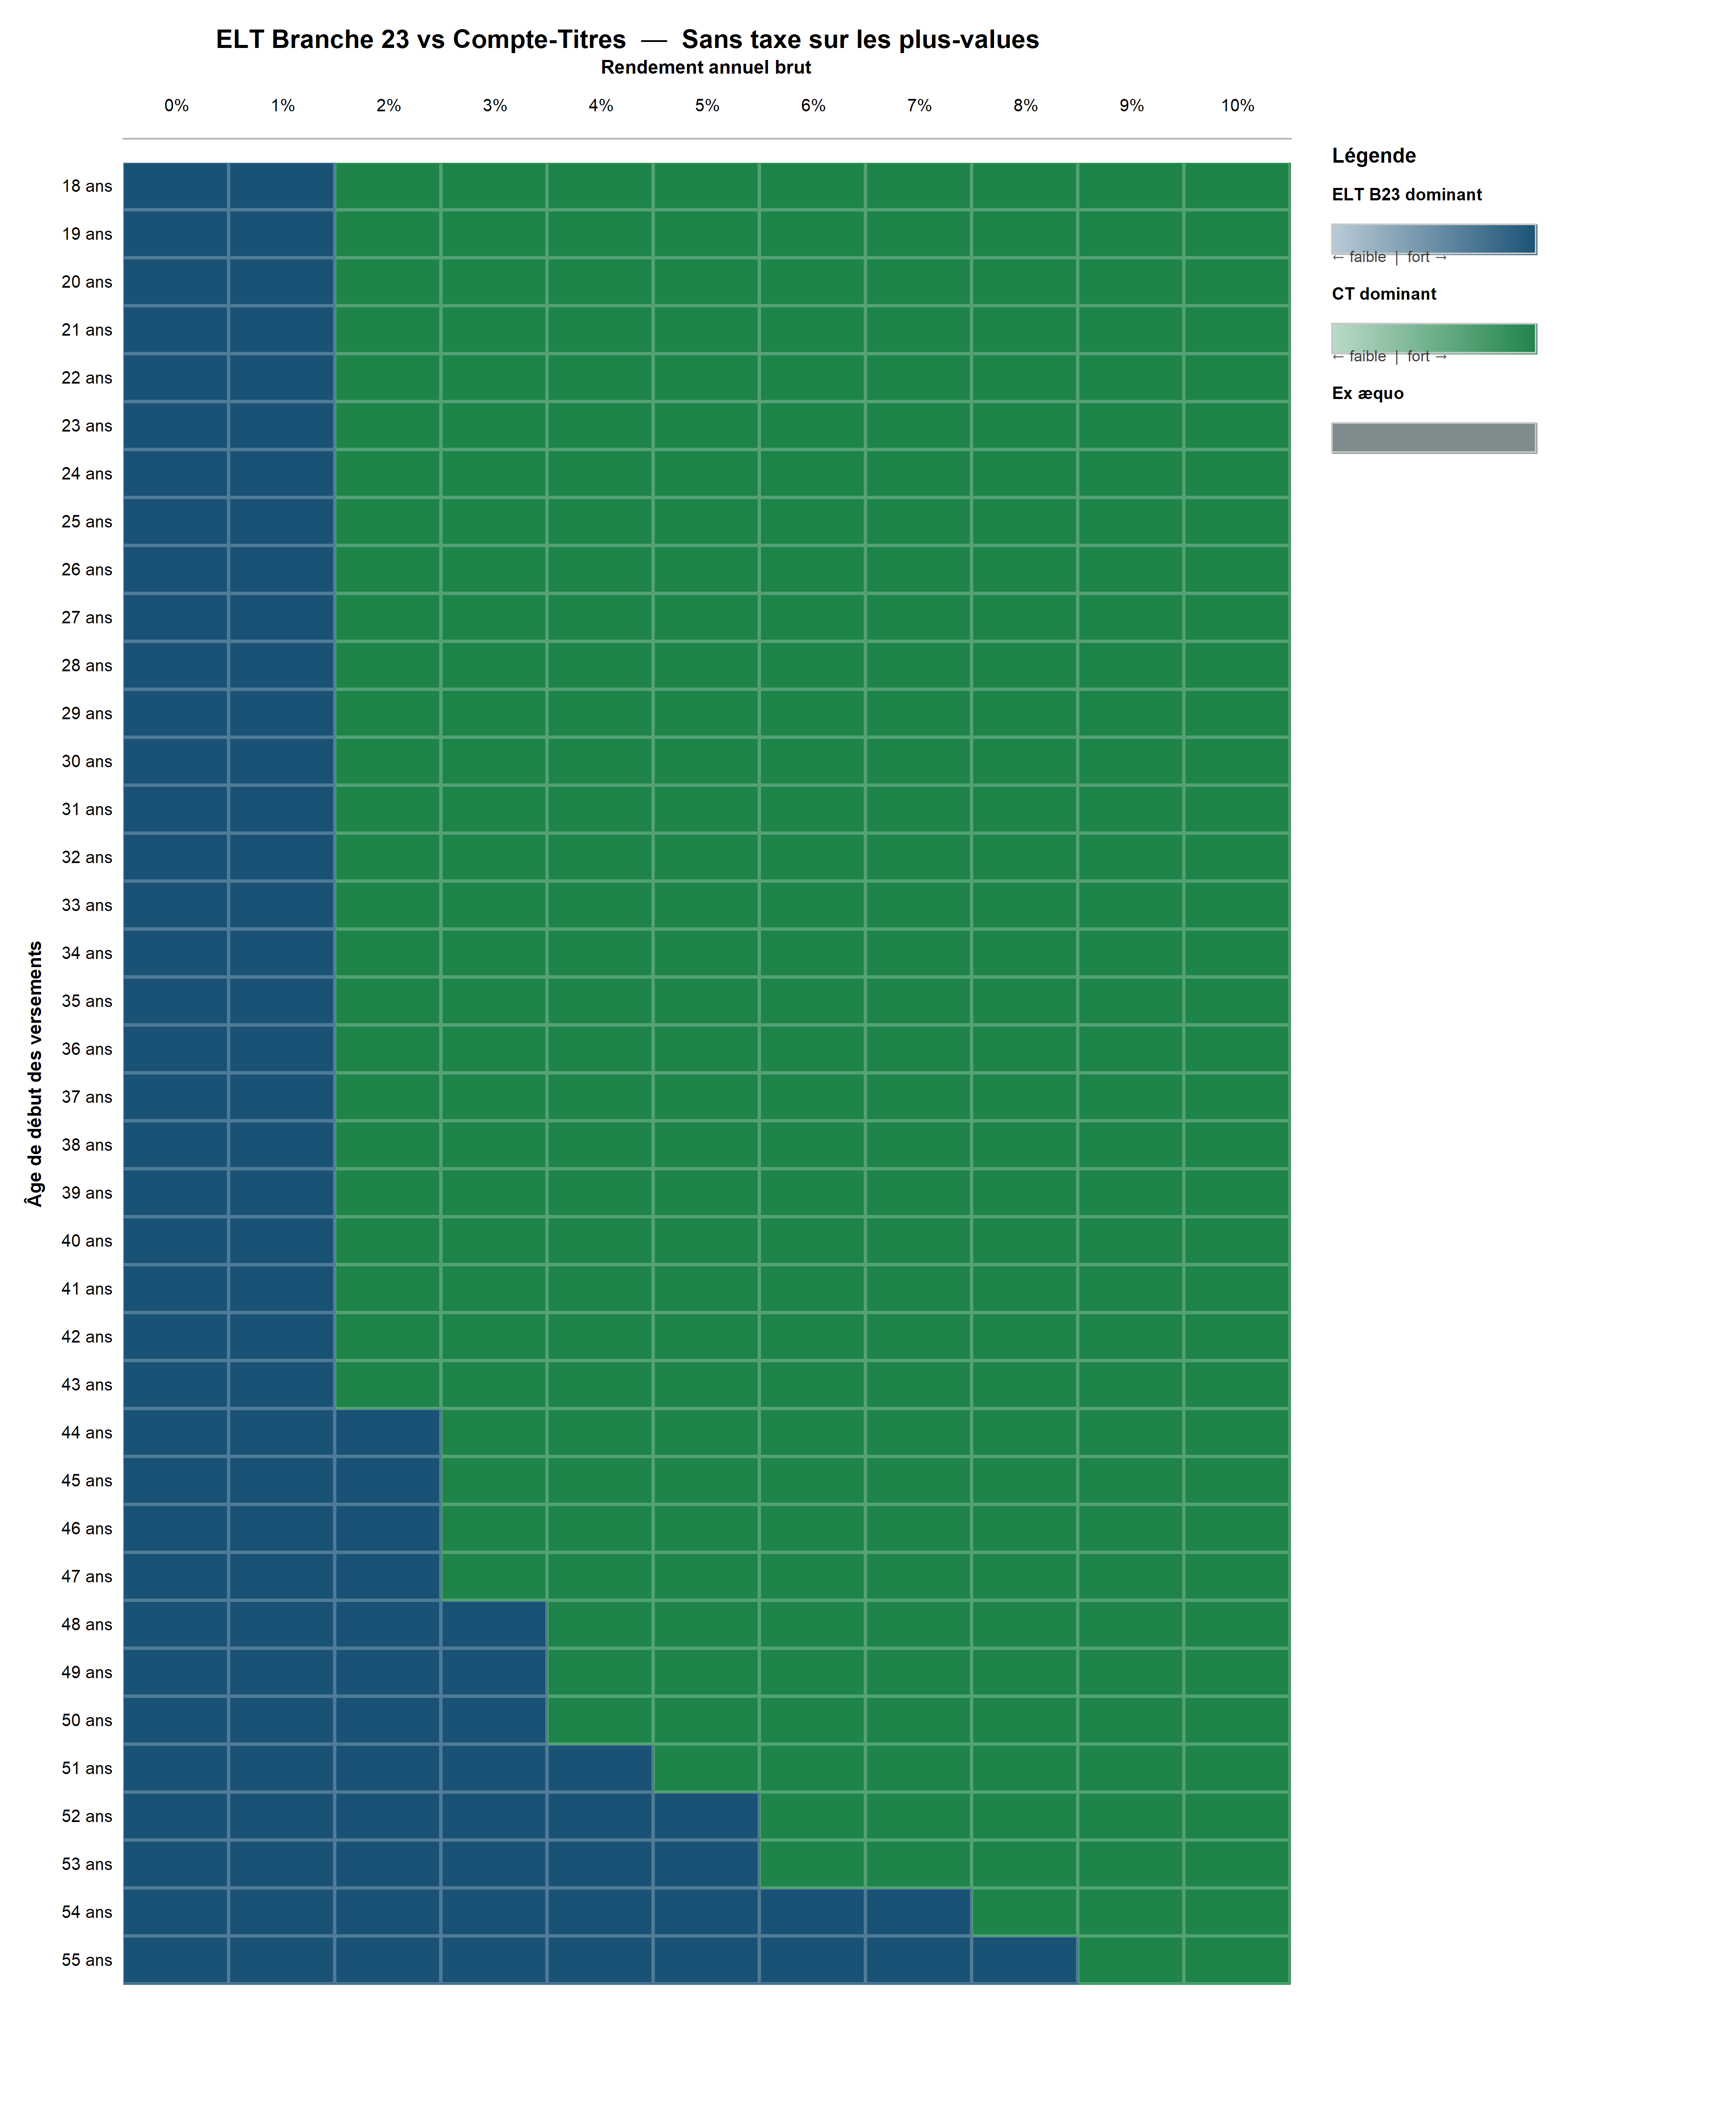
\includegraphics[width=0.5\textwidth]{media/elt_frais_reel_sans_taxe.png}
  \caption{Dominance ELT\,/\,CT --- Scénario~B, sans taxe sur les plus-values.
           Les cellules bleues indiquent la dominance de l'ELT à 100\,\%~;
           les cellules vertes indiquent la dominance du CT à 100\,\%.
           L'intensité de couleur reflète la force de la dominance.}
  \label{fig:elt_frais_reel_sans_taxe}
\end{figure}

La heatmap montre que le compte-titres l'emporte dans la majorité des
combinaisons simulées. L'ELT ne s'impose que dans une zone limitée,
correspondant aux rendements très faibles et à certains horizons courts.
À 0\,\% et 1\,\% de rendement, il l'emporte pour tous les âges~; à 2\,\%,
de 44 à 55~ans~; à 3\,\%, de 48 à 55~ans~; à 8\,\%, uniquement à partir
de 55~ans. Dès 9\,\%, le compte-titres l'emporte quelle que soit la date
de début. \hl{avant peut être réduire car 
on répète ce qu il y a sur le graph} Il ressort par ailleurs qu'au sein d'une même cellule, un seul instrument
domine sur l'intégralité de la plage de versements, sans aucun seuil de
croisement interne.

Plusieurs effets jouant simultanément en défaveur de l'ELT expliquent cette dominance
majoritaire des comptes-titres. 
La taxe sur les opérations d'assurance de 2\,\% et
les frais d'entrée de 2,83\,\% 
réduisent d'emblée la part du versement effectivement investie. 
Les frais de gestion
annuels de 2,34\,\% s'accumulent ensuite sur une réserve croissante.
 À cela s'ajoute la taxe anticipative de 10\,\%
prélevée sur la réserve constituée à 60~ans, qui ampute le capital accumulé.
Passé un certain horizon, ces coûts dépassent l'ensemble des économies fiscales
réalisées sur la période.
L'avantage fiscal annuel de l'ELT, plafonné à 735~€, ne suffit donc
pas à contrebalancer l'accumulation de ces coûts dès lors que le
rendement est élevé et l'horizon suffisamment long.

L'ELT l'emporte dans les situations où ces mécanismes n'ont pas le temps
ou le rendement suffisant pour jouer pleinement. À 0\,\% et 1\,\%, le
rendement est trop faible pour que le compte-titres génère un capital
significatif~; les économies fiscales annuelles de l'ELT prennent alors
le dessus sans peine. Aux rendements plus élevés, l'ELT reste gagnant
uniquement sur les horizons relativement courts. Avec peu d'années devant eux, les intérêts composés n'ont pas eu le
temps de s'accumuler, ni dans le compte-titres ni dans la branche~23.
Du côté du compte-titres, cela signifie qu'il n'a pas encore eu
l'occasion de creuser l'écart. Du côté de l'ELT, une réserve encore
modeste signifie que ni les frais ni les taxes 
ne pèsent encore significativement. Les économies fiscales
annuelles, perçues dès le premier versement, pèsent ainsi
proportionnellement plus lourd que tous les autres effets.

\hl{sans oublier en fait que les économies fiscales sont capitalisées à taux sans risque
et donc très favorable aux horizons longs mais dans le ou on ne capitaliserait pas
ce ne serait surement pas aussi écrasant même si la tendance serait quand meme là}

\subsubsection*{Incidence de la taxe sur les plus-values de 2026}

La figure~\ref{fig:elt_frais_reel_avec_taxe} reprend les mêmes simulations en
supposant que le compte-titres supporte la taxe de 10\,\% sur les
plus-values introduite en 2026.

\begin{figure}[H]
  \centering
  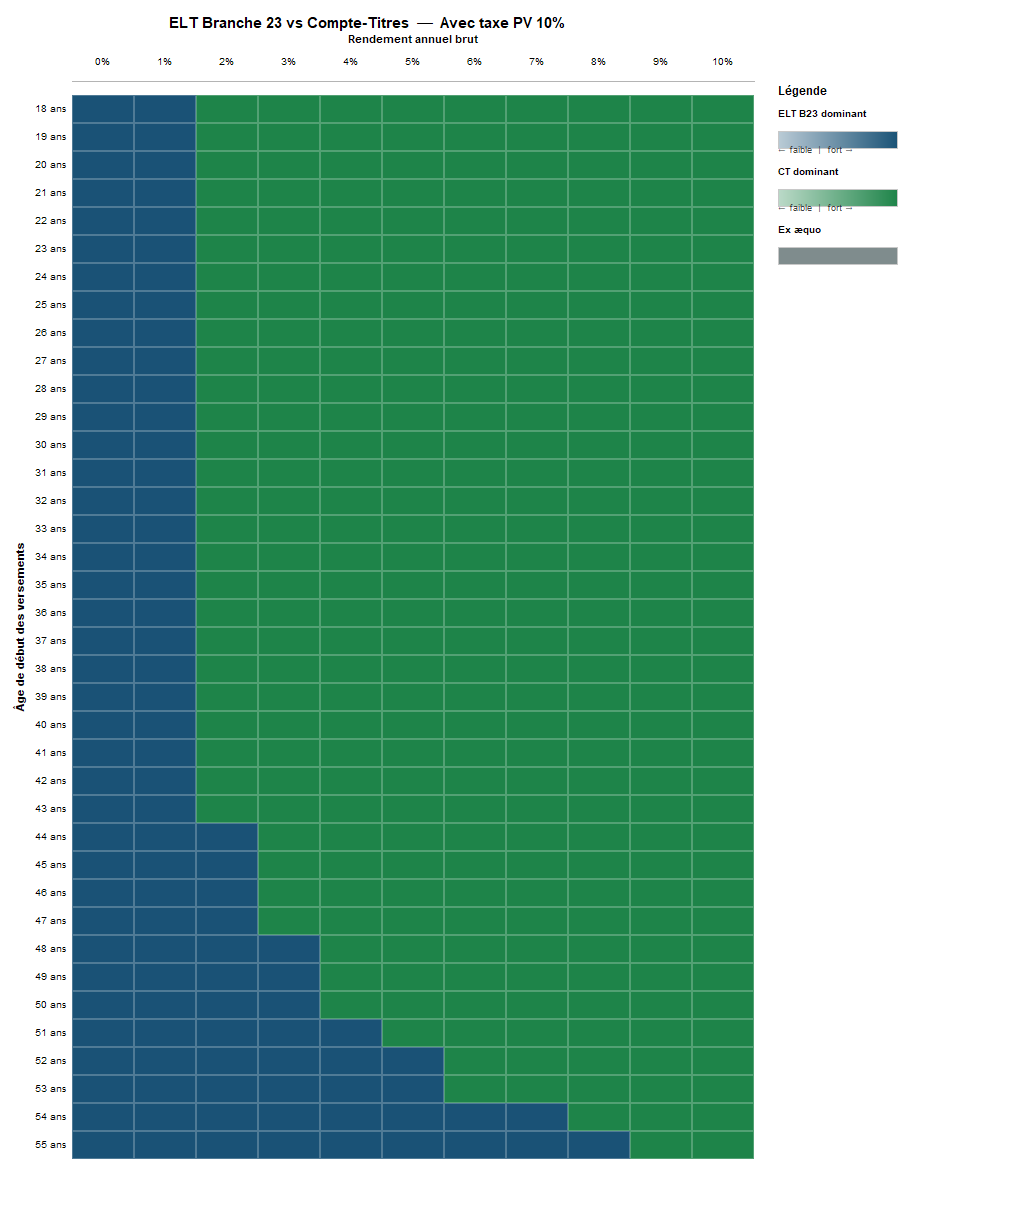
\includegraphics[width=0.5\textwidth]{media/elt_frais_reel_avec_taxe.png}
  \caption{Dominance ELT\,/\,CT --- Scénario~B, avec taxe sur les
           plus-values de 10\,\%.}
  \label{fig:elt_frais_reel_avec_taxe}
\end{figure}

Les deux heatmaps sont visuellement identiques. La taxe réduit légèrement
les marges du compte-titres aux rendements les plus élevés, ce qui est
perceptible dans les données brutes, mais elle ne déplace aucun seuil et
ne renverse aucun résultat. En pratique, la réforme de 2026 ne change pas
les conclusions dans ce scénario~; c'est le niveau des frais qui détermine
l'issue, davantage que la fiscalité à la sortie.

\hl{effectivement on voit l impact dans les données brutes mais uniquement pour les montants
impactés par taxe sur les plus values, par exemple pour montant dont plus value est
inférieur à 15000 forcément pas impact mais je ne pense pas qu'il faille mentionner,
surement que ça doit juste être implicite}

%--------------------------------------------------------------------------
\subsection{Scénarios~A et~C --- Traitement commun}
\label{sec:resultats_elt_AC}

Le scénario~A supprime tous les frais des deux côtés, de façon à observer
l'avantage fiscal de l'ELT à l'état pur. Le scénario~C fait l'inverse~: il
applique les mêmes frais au compte-titres qu'à l'ELT (2,83\,\% à l'entrée
et 2,34\,\% de gestion), ce qui neutralise l'écart tarifaire. Les heatmaps
correspondantes sont présentées en annexe
(figures~\ref{fig:elt_frais_0_sans_taxe}, \ref{fig:elt_frais_0_avec_taxe},
\ref{fig:elt_frais_majore_sans_taxe} et~\ref{fig:elt_frais_majore_avec_taxe}).

\hl{tout ça on dit déjà, peut être retirer si trop redondant}

\subsubsection*{Résultats principaux}

Pour le scénario~A sans taxe sur les plus-values, l'ELT domine
presque partout. Le compte-titres ne l'emporte que dans les zones à rendement
élevé et horizon long~: de 18 à 27~ans à 7\,\%, de 18 à 33~ans à 8\,\%,
de 18 à 38~ans à 9\,\% et de 18 à 41~ans à 10\,\%. Ces exceptions
correspondent à des situations où la taxe sur les opérations d'assurance de
2\,\%, conjuguée à la taxe anticipative de
10\,\%, finit par excéder
l'ensemble des réductions d'impôt cumulées sur toute la durée du contrat.
C'est en quelque sorte la limite inhérente au régime fiscal de l'ELT,
indépendante du niveau des frais.

Lorsque l'on égalise les frais (scénario~C), ces zones se réduisent
nettement~ \hl{par rapport à B}: il ne reste que quatre bandes, à 7\,\% de 18 à 32 ans, à 8\,\% de 18 à 39 ans, à 9\,\% de 18 à 44~ans et à
10\,\% de 18 à 46~ans. L'extension est en réalité significative~: en passant du scénario~A
au scénario~C, les zones où le compte-titres l'emporte s'élargissent.
Ce résultat peut sembler paradoxal puisque les frais sont désormais
nominalement identiques des deux côtés, mais il s'explique par la façon
dont ils sont prélevés~: pour le compte-titres, les frais sont certes
calculés sur le capital accumulé, mais ils sont supportés en dehors du
portefeuille, si bien que l'intégralité du capital continue à se
capitaliser~; pour l'épargne long terme, ces mêmes frais sont en revanche
déduits directement du capital accumulé, réduisant ainsi la base de
composition à chaque période. À taux nominalement égal, le compte-titres
conserve donc un avantage structurel de capitalisation que le scénario~C
met précisément en évidence.

\subsubsection*{Incidence de la taxe sur les plus-values}

Lorsque la taxe de 10\,\% sur les plus-values s'applique au compte-titres,
les quelques cellules encore dominées par celui-ci font apparaître un seuil
de croisement à des montants très bas~: entre 73~€ et 218~€ par an dans le
scénario~A. En dessous de ces
montants, le compte-titres conserve encore un léger avantage~; au-delà,
l'ELT reprend la tête. \hl{Ces seuils sont tellement faibles par rapport au
plafond de versement de 2\,450~€ que, pour tout versement d'un niveau
économiquement courant, l'ELT est gagnant dès lors que les deux instruments
sont logés à la même enseigne fiscale à la sortie. Le fait que ces seuils
soient comparables entre les scénarios~A et~C confirme qu'ils dépendent de
la structure fiscale des deux instruments et non du niveau des frais.}

\hl{pour le scenario C c est juste que la taxe sur les plus values vient grignoter
des places par rapport au cas sans taxe sur les pv}

\subsubsection*{Ce que la comparaison des trois scénarios révèle}

En mettant les trois scénarios côte à côte, on peut attribuer un rôle précis
à chaque variable. Le passage de~A à~B, c'est-à-dire l'ajout des frais
moyens du marché à l'ELT sans modifier ceux du compte-titres, suffit à renverser
presque entièrement l'avantage fiscal de l'ELT. Le passage de~B à~C,
qui ajoute les mêmes frais au compte-titres, le restaure largement, sauf
aux rendements les plus élevés sur certains horizons plus longs, où les
taxes restent le facteur limitant. La taxe sur les plus-values de 2026, quant à elle, produit des effets
différenciés selon le scénario. Dans le scénario~B, elle améliore
légèrement la position de l'ELT sans en renverser la hiérarchie~: le
compte-titres demeure dominant sur l'essentiel de la plage. Dans les
scénarios~A et~C en revanche, elle fait basculer la hiérarchie en faveur
de l'ELT, qui devient dominant sur toute la plage, à l'exception
des quelques cellules présentant un seuil de croisement à des montants très
bas.
\hl{je ne sais pas si c est nécessaire, en plus c est vraiment obvious + plus
accurate vu que j ai changé une partie}

\newpage

%==========================================================================
\section{Résultats~: épargne-pension (branche~23) versus compte-titres}
\label{sec:resultats_ep}

Les simulations comparent, pour chaque combinaison d'âge de début et de
rendement annuel brut, le capital final net à l'échéance de l'EP et du
compte-titres sur l'ensemble de la plage de versements (de 1~€ à
1\,350~€ par an). Une différence fondamentale distingue cependant l'EP de l'ELT.
Son taux de réduction d'impôt n'est pas uniforme~: il s'applique à 30\,\%
pour les versements jusqu'à 1\,050~€, puis retombe à 25\,\% pour la
tranche allant jusqu'au plafond de 1\,350~€. Ce palier génère, dans de
nombreuses cellules, un seuil de croisement structurel autour de 1\,050~€
par an.

\hl{encore une fois redondant}

%--------------------------------------------------------------------------
\subsection{Scénario~B --- Frais réalistes (cas central)}
\label{sec:resultats_ep_B}

\subsubsection*{Frontière de dominance sans taxe sur les plus-values}

\begin{figure}[H]
  \centering
  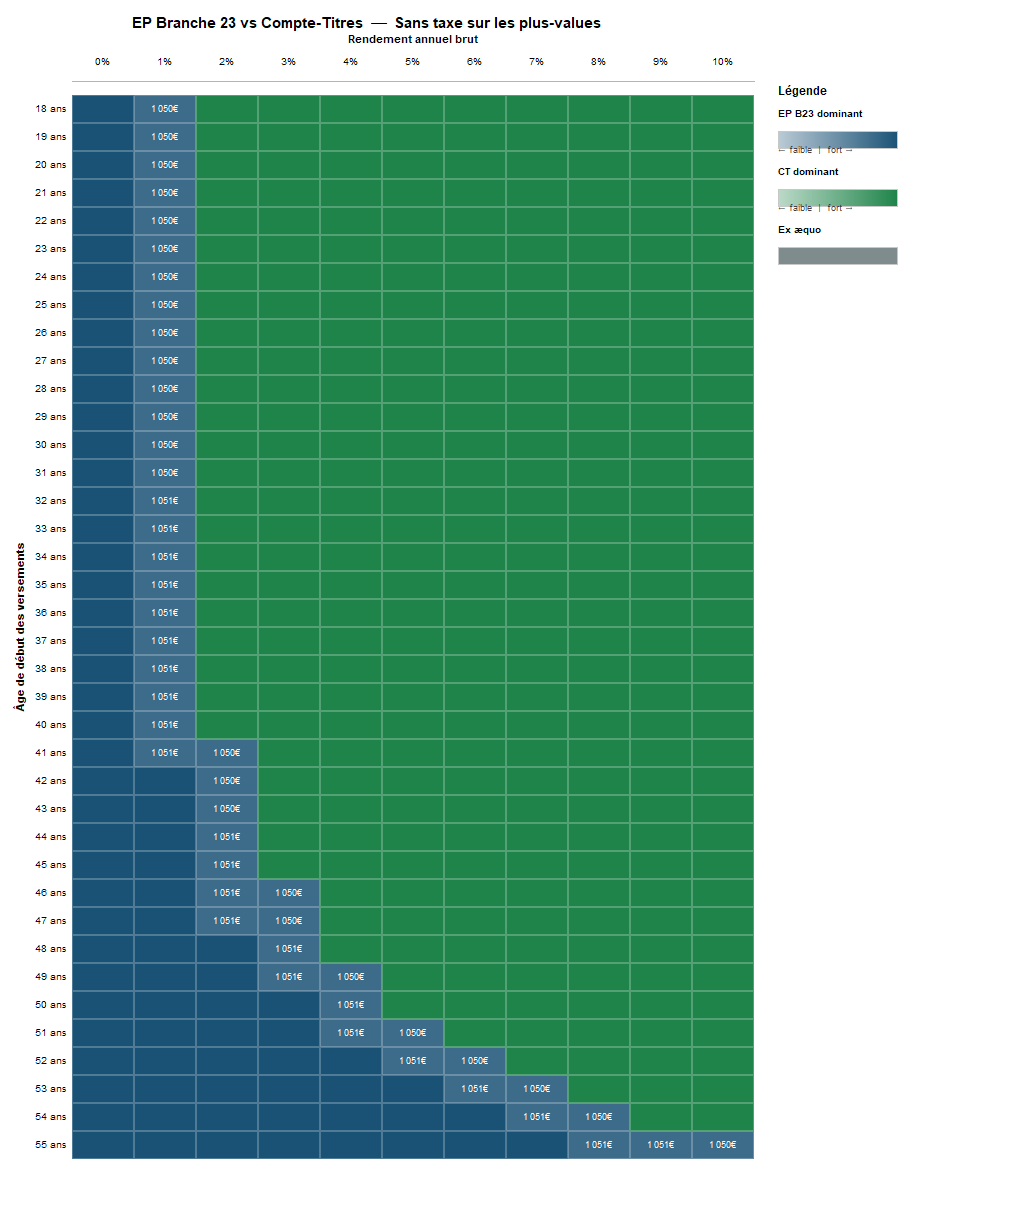
\includegraphics[width=0.5\textwidth]{media/ep_frais_reel_sans_taxe.png}
  \caption{Dominance EP\,/\,CT --- Scénario~B, sans taxe sur les plus-values.
           Les cellules bleues indiquent la dominance de l'EP~;
           les cellules vertes indiquent la dominance du CT.
           L'intensité de couleur reflète la force de la dominance.}
  \label{fig:ep_frais_reel_sans_taxe}
\end{figure}

La heatmap présente deux types de zones bleues bien distincts. Les cellules
bleu foncé, où l'EP domine sur l'intégralité de la plage de versements, se
concentrent aux rendements faibles et aux horizons courts. À 0\,\%, l'EP
l'emporte pour tous les âges de début~; à 1\,\%, à partir de 42~ans~; à
2\,\%, à partir de 48~ans~; à 3\,\%, à partir de 50~ans~; à 4\,\%, à
partir de 52~ans~; à 5\,\%, à partir de 53~ans~; à 6\,\%, à partir de
54~ans~; à 7\,\%, à 55~ans seulement. Dès 8\,\%, aucune cellule ne
présente de dominance totale de l'EP.

Les cellules bleu clair révèlent une dominance partielle, structurellement
absente dans le cas de l'ELT. L'EP s'impose jusqu'au versement annuel de
1\,050 ou 1\,051~€, au-delà duquel le compte-titres reprend la tête. Ce
seuil traduit directement le palier de la réduction d'impôt de l'EP.
Passé 1\,050~€, le taux retombe à 25\,\% et l'avantage fiscal s'érode
suffisamment pour que le compte-titres l'emporte. Ces cellules à dominance
partielle s'étendent de 18 à 41~ans à 1\,\%, de 41 à 47~ans à 2\,\%, de
46 à 49~ans à 3\,\%, de 49 à 51~ans à 4\,\%, de 51 à 52~ans à 5\,\%, de
52 à 53~ans à 6\,\%, de 53 à 54~ans à 7\,\%, de 54 à 55~ans à 8\,\%, et
à 55~ans uniquement pour les rendements de 9\,\% et 10\,\%.

Le compte-titres l'emporte dans ce scénario pour les mêmes raisons
structurelles que dans le cas de l'ELT, à savoir sa structure de coûts
plus légère aux rendements élevés et sur les longues durées. La
caractéristique propre à l'EP est le seuil à 1\,050~€, absent dans
l'analyse de l'ELT qui applique un taux uniforme de 30\,\%. En dessous de
ce palier, l'EP bénéficie du même taux de 30\,\% que l'ELT~; au-delà, la
baisse à 25\,\% érode l'avantage fiscal au point que le compte-titres
l'emporte même dans des cellules où l'EP dominait encore jusqu'à ce
versement \hl{cette phrase est formulée bizarrement}. Comparé à l'ELT, l'EP présente des zones de dominance totale
légèrement plus étendues aux rendements intermédiaires, jusqu'à 7\,\%
pour les horizons les plus courts, là où l'ELT n'a plus de dominance
totale dès 4\,\%. Cette différence tient à l'absence de taxe sur les
opérations d'assurance dans l'EP et à son taux de taxe anticipative plus
faible, 8\,\% contre 10\,\%.

\subsubsection*{Incidence de la taxe sur les plus-values de 2026}

\begin{figure}[H]
  \centering
  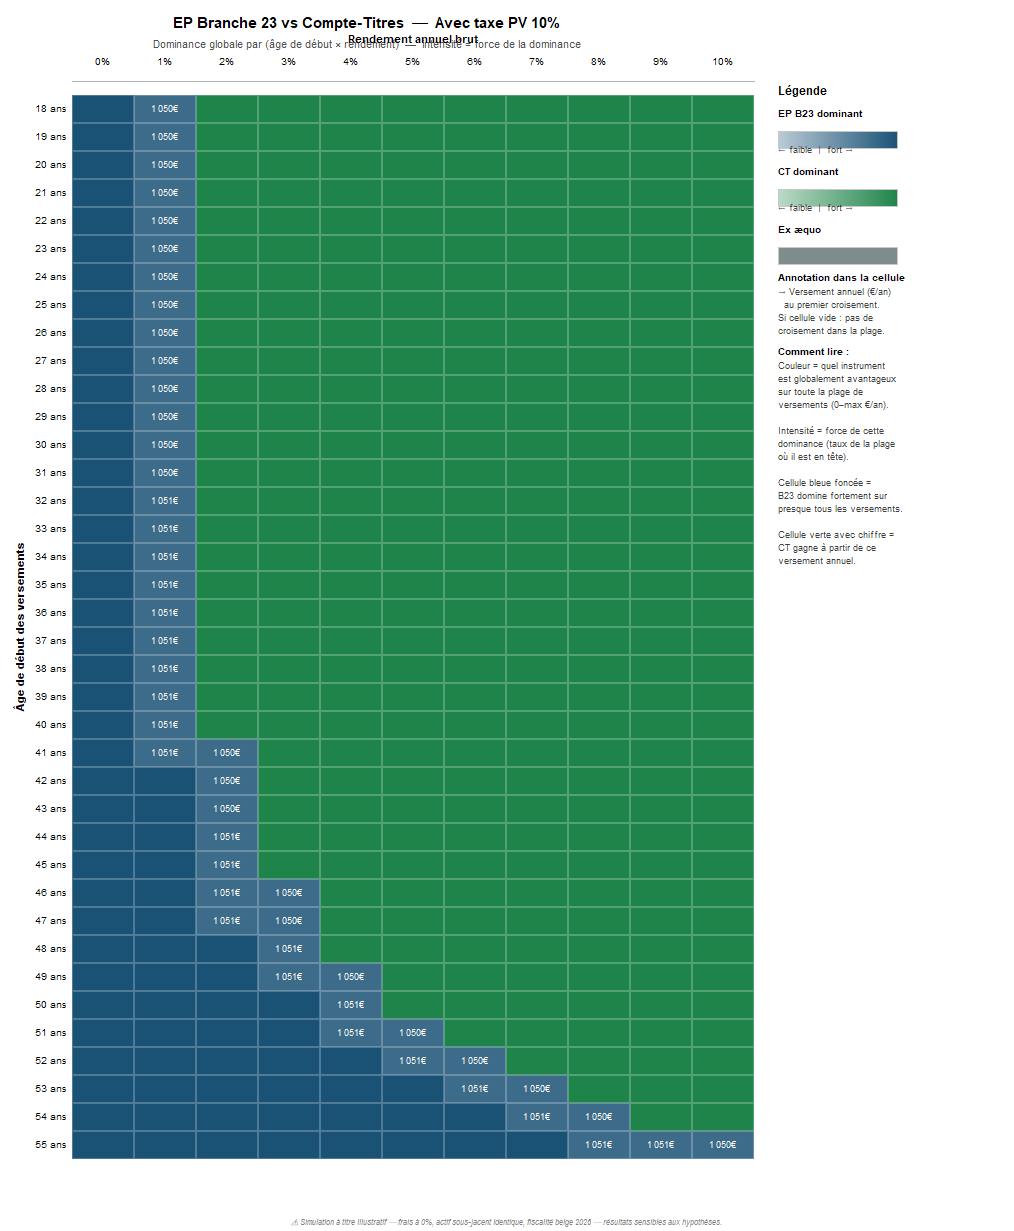
\includegraphics[width=0.5\textwidth]{media/ep_frais_reel_avec_taxe.png}
  \caption{Dominance EP\,/\,CT --- Scénario~B, avec taxe sur les
           plus-values de 10\,\%.}
  \label{fig:ep_frais_reel_avec_taxe}
\end{figure}

La heatmap avec taxe sur les plus-values est visuellement identique à la
précédente. Comme pour l'ELT dans le scénario~B, la réforme de 2026
réduit légèrement les marges du compte-titres aux rendements les plus
élevés, ce qui est perceptible dans les données brutes, mais elle ne
déplace aucun seuil et ne renverse aucun résultat. La structure des frais
reste le facteur déterminant, davantage que la fiscalité à la sortie.

%--------------------------------------------------------------------------
\subsection{Scénarios~A et~C --- Traitement commun}
\label{sec:resultats_ep_AC}

Les heatmaps des scénarios~A et~C sont présentées en annexe.

\subsubsection*{Résultats principaux}

Pour le scénario~A sans taxe sur les plus-values, l'EP domine massivement.
Le compte-titres ne l'emporte à 100\,\% que dans les zones à rendement
élevé et horizon long~: de 18 à 23~ans à 8\,\%, de 18 à 29~ans à 9\,\%
et de 18 à 34~ans à 10\,\%. Des seuils de croisement autour de 1\,050~€
subsistent dans les bandes adjacentes, de 24 à 28~ans à 8\,\%, de 30 à
33~ans à 9\,\% et de 35 à 37~ans à 10\,\%. Ces zones d'exception sont
plus restreintes que celles observées pour l'ELT dans le même scénario,
ce qui s'explique par l'absence de taxe sur les opérations d'assurance
dans l'EP et par son taux de taxe anticipative plus faible.

Lorsque l'on égalise les frais (scénario~C), les zones d'exception se
réduisent davantage encore \hl{par rapport à B}. Le compte-titres domine à 100\,\% 
de 18 à 28 ans pour un rendmeent de 7\,\%, de 18 à 37 ans pour un rendmeent de 8\,\%,
de 18 à 41 ans pour un rendmeent de 9\,\%,
de 18 à 44~ans à 10\,\%, tandis qu'un seuil de croisement subsiste de
18 à 20~ans à 9\,\% et de 25 à 29~ans à 10\,\% \hl{corriger ici}. Le recul par rapport au
scénario~B confirme une nouvelle fois que la différence de frais, bien
plus que la fiscalité, est le facteur déterminant dans les conditions
réelles de marché.

\subsubsection*{Incidence de la taxe sur les plus-values}

Lorsque la taxe de 10\,\% sur les plus-values s'applique au compte-titres,
les rares cellules encore favorables à celui-ci présentent des seuils très
bas. Dans le scénario~A, l'EP reprend la tête dès 33~€ pour un âge de
début de 18~ans à 10\,\% de rendement, et dès 90~€ pour un âge de début
de 34~ans au même rendement~; en dessous de ces montants, le compte-titres
conserve encore un léger avantage. Dans le scénario~C, les seuils
correspondants s'établissent à 55~€ pour un âge de début de 18~ans et à
70~€ pour 24~ans, toujours à 10\,\%. Ces niveaux sont si faibles par
rapport au plafond de versement de 1\,350~€ que, pour tout versement d'un
montant économiquement courant, l'EP est gagnant dès lors que les deux
instruments supportent les mêmes charges à l'entrée et à la sortie.

\hl{corriger, mais au final juste grignotement}

\subsubsection*{Ce que la comparaison des trois scénarios révèle}

Les conclusions rejoignent celles tirées pour l'ELT. Le passage du
scénario~A au scénario~B, qui introduit les frais moyens du marché dans
l'EP sans en faire autant pour le compte-titres, renverse largement la
balance en faveur du compte-titres. Le passage de~B à~C, qui soumet le
compte-titres aux mêmes frais, la restaure presque entièrement. La taxe
sur les plus-values de 2026 produit un effet marginal dans le scénario~B,
tandis qu'elle fait basculer les dernières cellules favorables au
compte-titres dans les scénarios~A et~C, sauf à des niveaux de versements
économiquement négligeables. La structure des frais, et non l'écart
fiscal, demeure le facteur déterminant dans les conditions réelles de
marché.

\hl{corriger}

\newpage
\pagestyle{empty}

\bibliographystyle{apacite}
\bibliography{references}

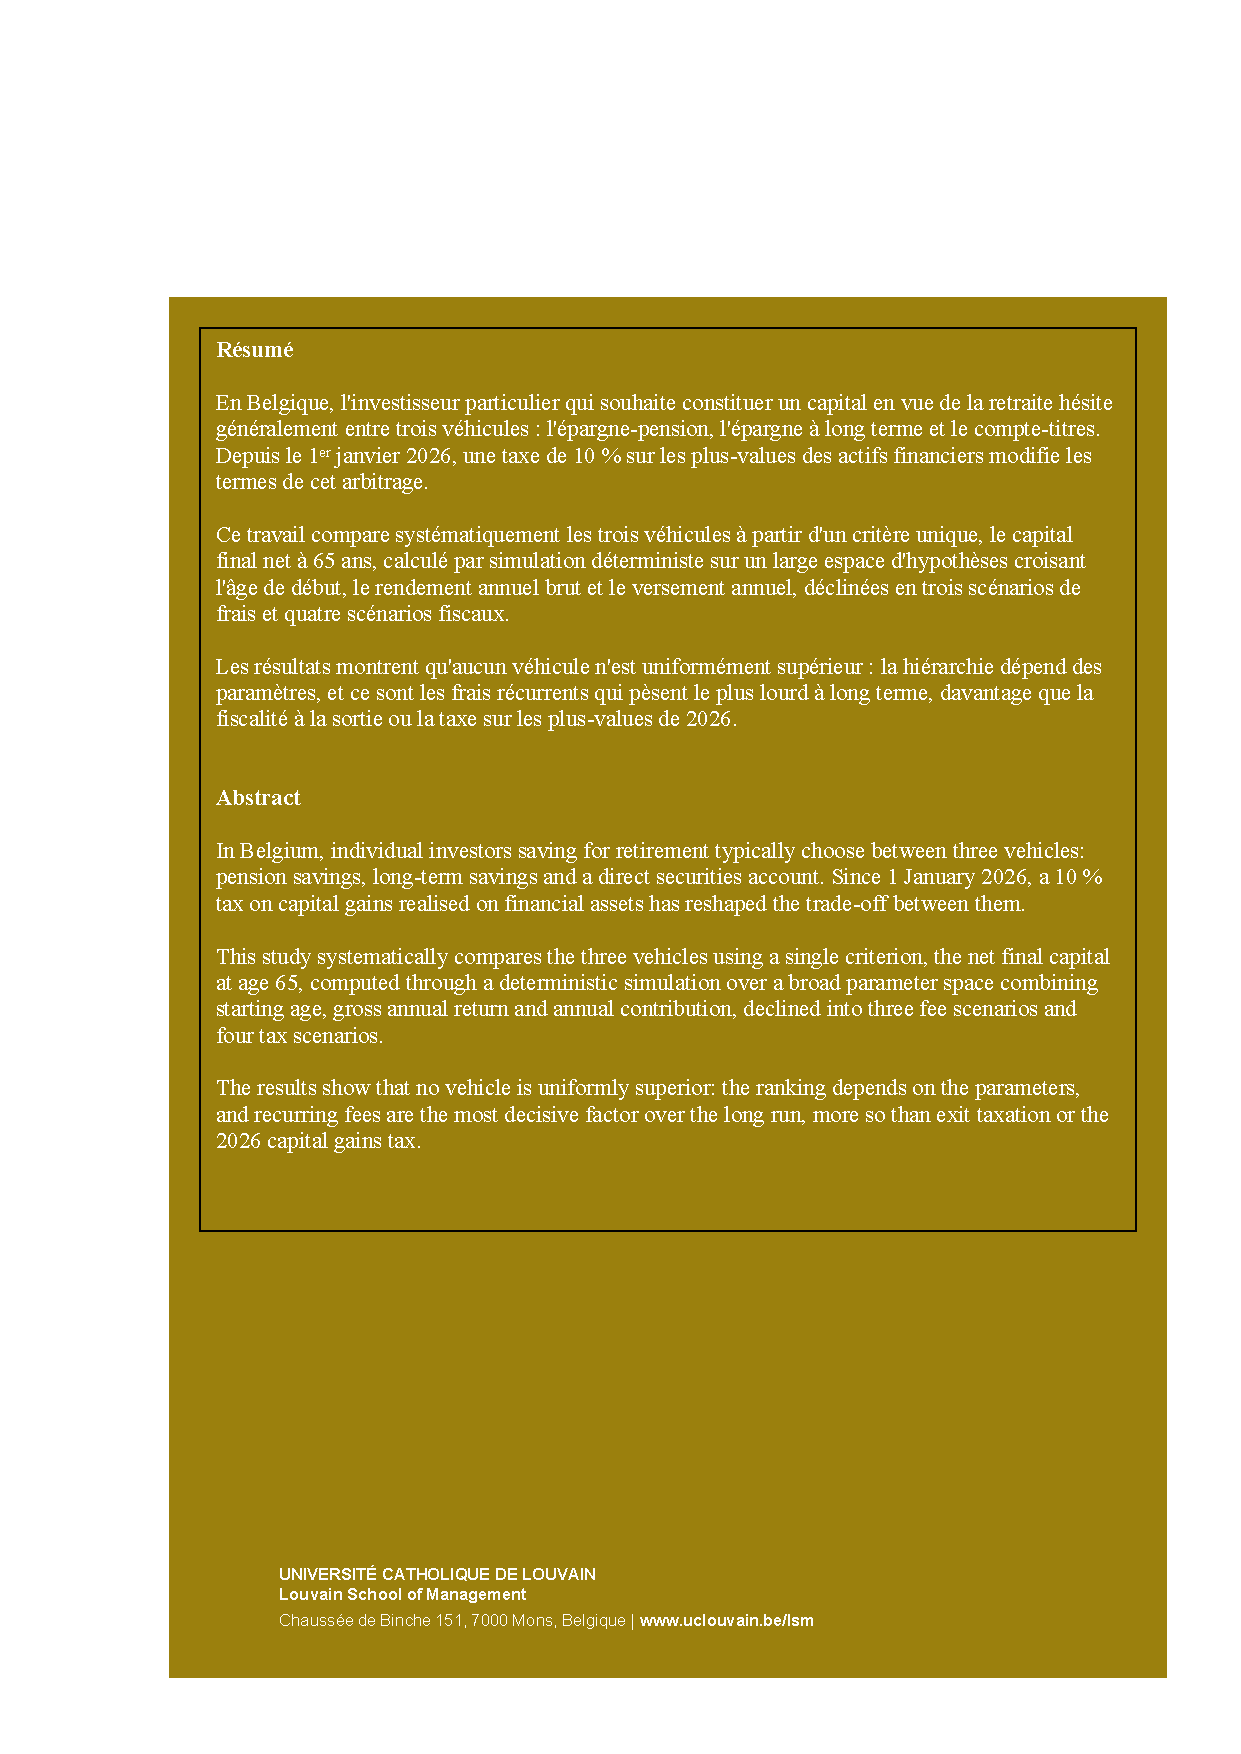
\includepdf[pages=-]{media/back.pdf}

\newpage
\pagestyle{empty}
\appendix

\section{Référentiel OLO belge utilisé pour la capitalisation}
\label{ann:olo}

\begin{table}[h!]
  \centering
  \caption{Référentiel OLO belge~: taux bruts et taux nets après précompte mobilier de 30\,\%}
  \label{tab:olo_referentiel}
  \begin{tabular}{ccc}
    \hline
    \textbf{Maturité (ans)} & \textbf{OLO brut (\%)} & \textbf{Taux net utilisé (\%)} \\
    \hline
     1 & 2,62 & 1,834 \\
     2 & 2,72 & 1,904 \\
     3 & 2,83 & 1,981 \\
     4 & 2,95 & 2,065 \\
     5 & 3,06 & 2,142 \\
     6 & 3,17 & 2,219 \\
     7 & 3,27 & 2,289 \\
     8 & 3,39 & 2,373 \\
     9 & 3,51 & 2,457 \\
    10 & 3,63 & 2,541 \\
    11 & 3,73 & 2,611 \\
    12 & 3,81 & 2,667 \\
    13 & 3,87 & 2,709 \\
    14 & 3,93 & 2,751 \\
    15 & 3,98 & 2,786 \\
    16 & 4,03 & 2,821 \\
    17 & 4,08 & 2,856 \\
    18 & 4,13 & 2,891 \\
    19 & 4,17 & 2,919 \\
    20 & 4,21 & 2,947 \\
    21 & 4,25 & 2,975 \\
    22 & 4,29 & 3,003 \\
    23 & 4,32 & 3,024 \\
    24 & 4,35 & 3,045 \\
    25 & 4,37 & 3,059 \\
    26 & 4,39 & 3,073 \\
    27 & 4,41 & 3,087 \\
    28 & 4,42 & 3,094 \\
    29 & 4,43 & 3,101 \\
    30 & 4,43 & 3,101 \\
    \hline
    \multicolumn{3}{l}{\small Au-delà de 30~ans, le taux net de l'année~30 (3,101\,\%) est appliqué.} \\
    \hline
  \end{tabular}
\end{table}

%==========================================================================
\section{Heatmaps ELT\,/\,CT --- Scénario~A (effet fiscal pur)}
\label{ann:heatmaps_A}

\begin{figure}[H]
  \centering
  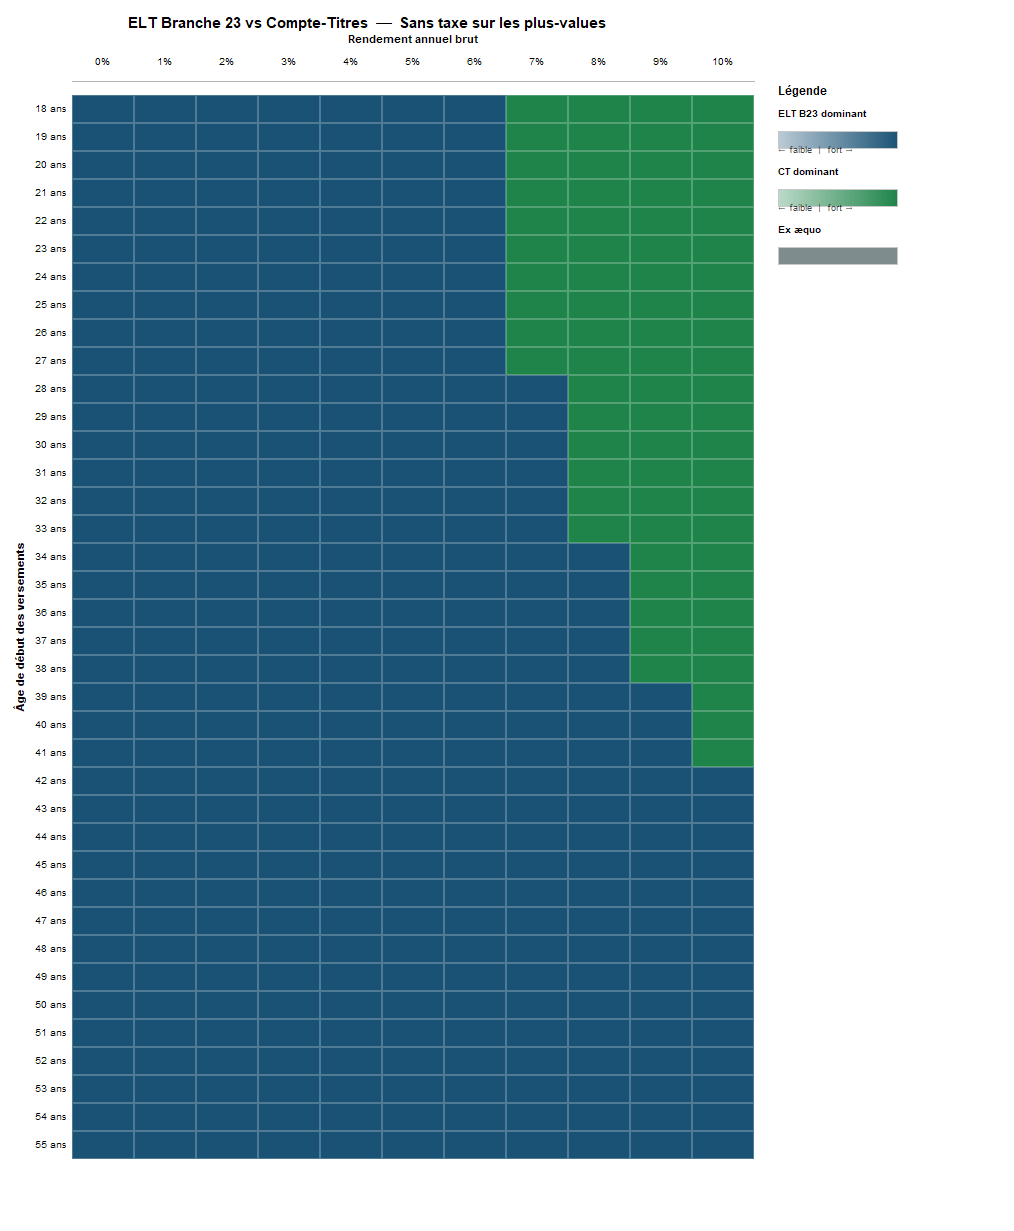
\includegraphics[width=\textwidth]{media/elt_frais_0_sans_taxe.png}
  \caption{Dominance ELT\,/\,CT --- Scénario~A (aucun frais), sans taxe sur les plus-values.}
  \label{fig:elt_frais_0_sans_taxe}
\end{figure}

\begin{figure}[H]
  \centering
  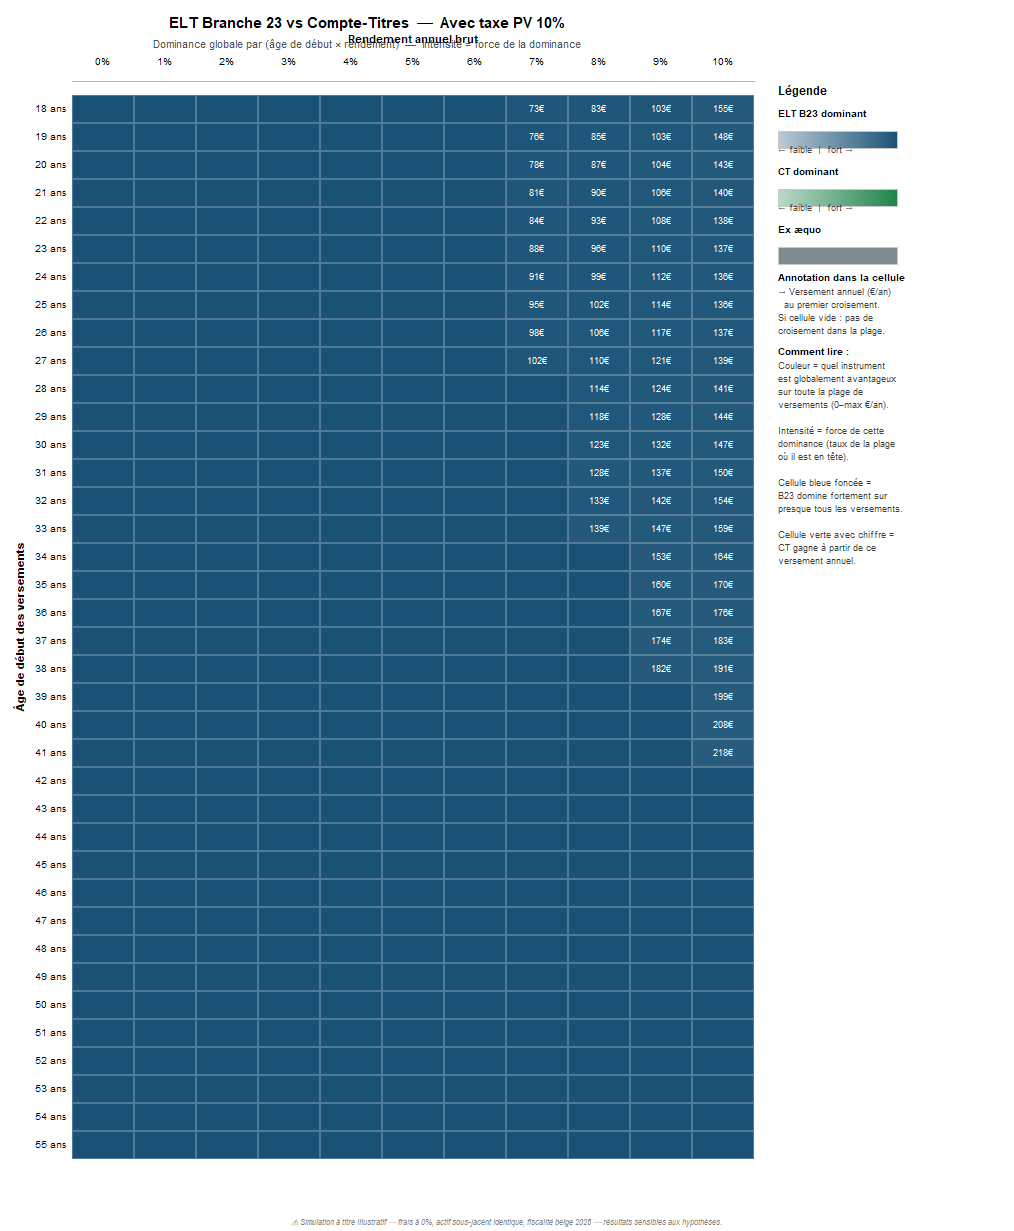
\includegraphics[width=\textwidth]{media/elt_frais_0_avec_taxe.png}
  \caption{Dominance ELT\,/\,CT --- Scénario~A (aucun frais), avec taxe sur les plus-values de 10\,\%.}
  \label{fig:elt_frais_0_avec_taxe}
\end{figure}

%==========================================================================
\section{Heatmaps ELT\,/\,CT --- Scénario~B (frais réalistes)}
\label{ann:heatmaps_elt_B}

\begin{figure}[H]
  \centering
  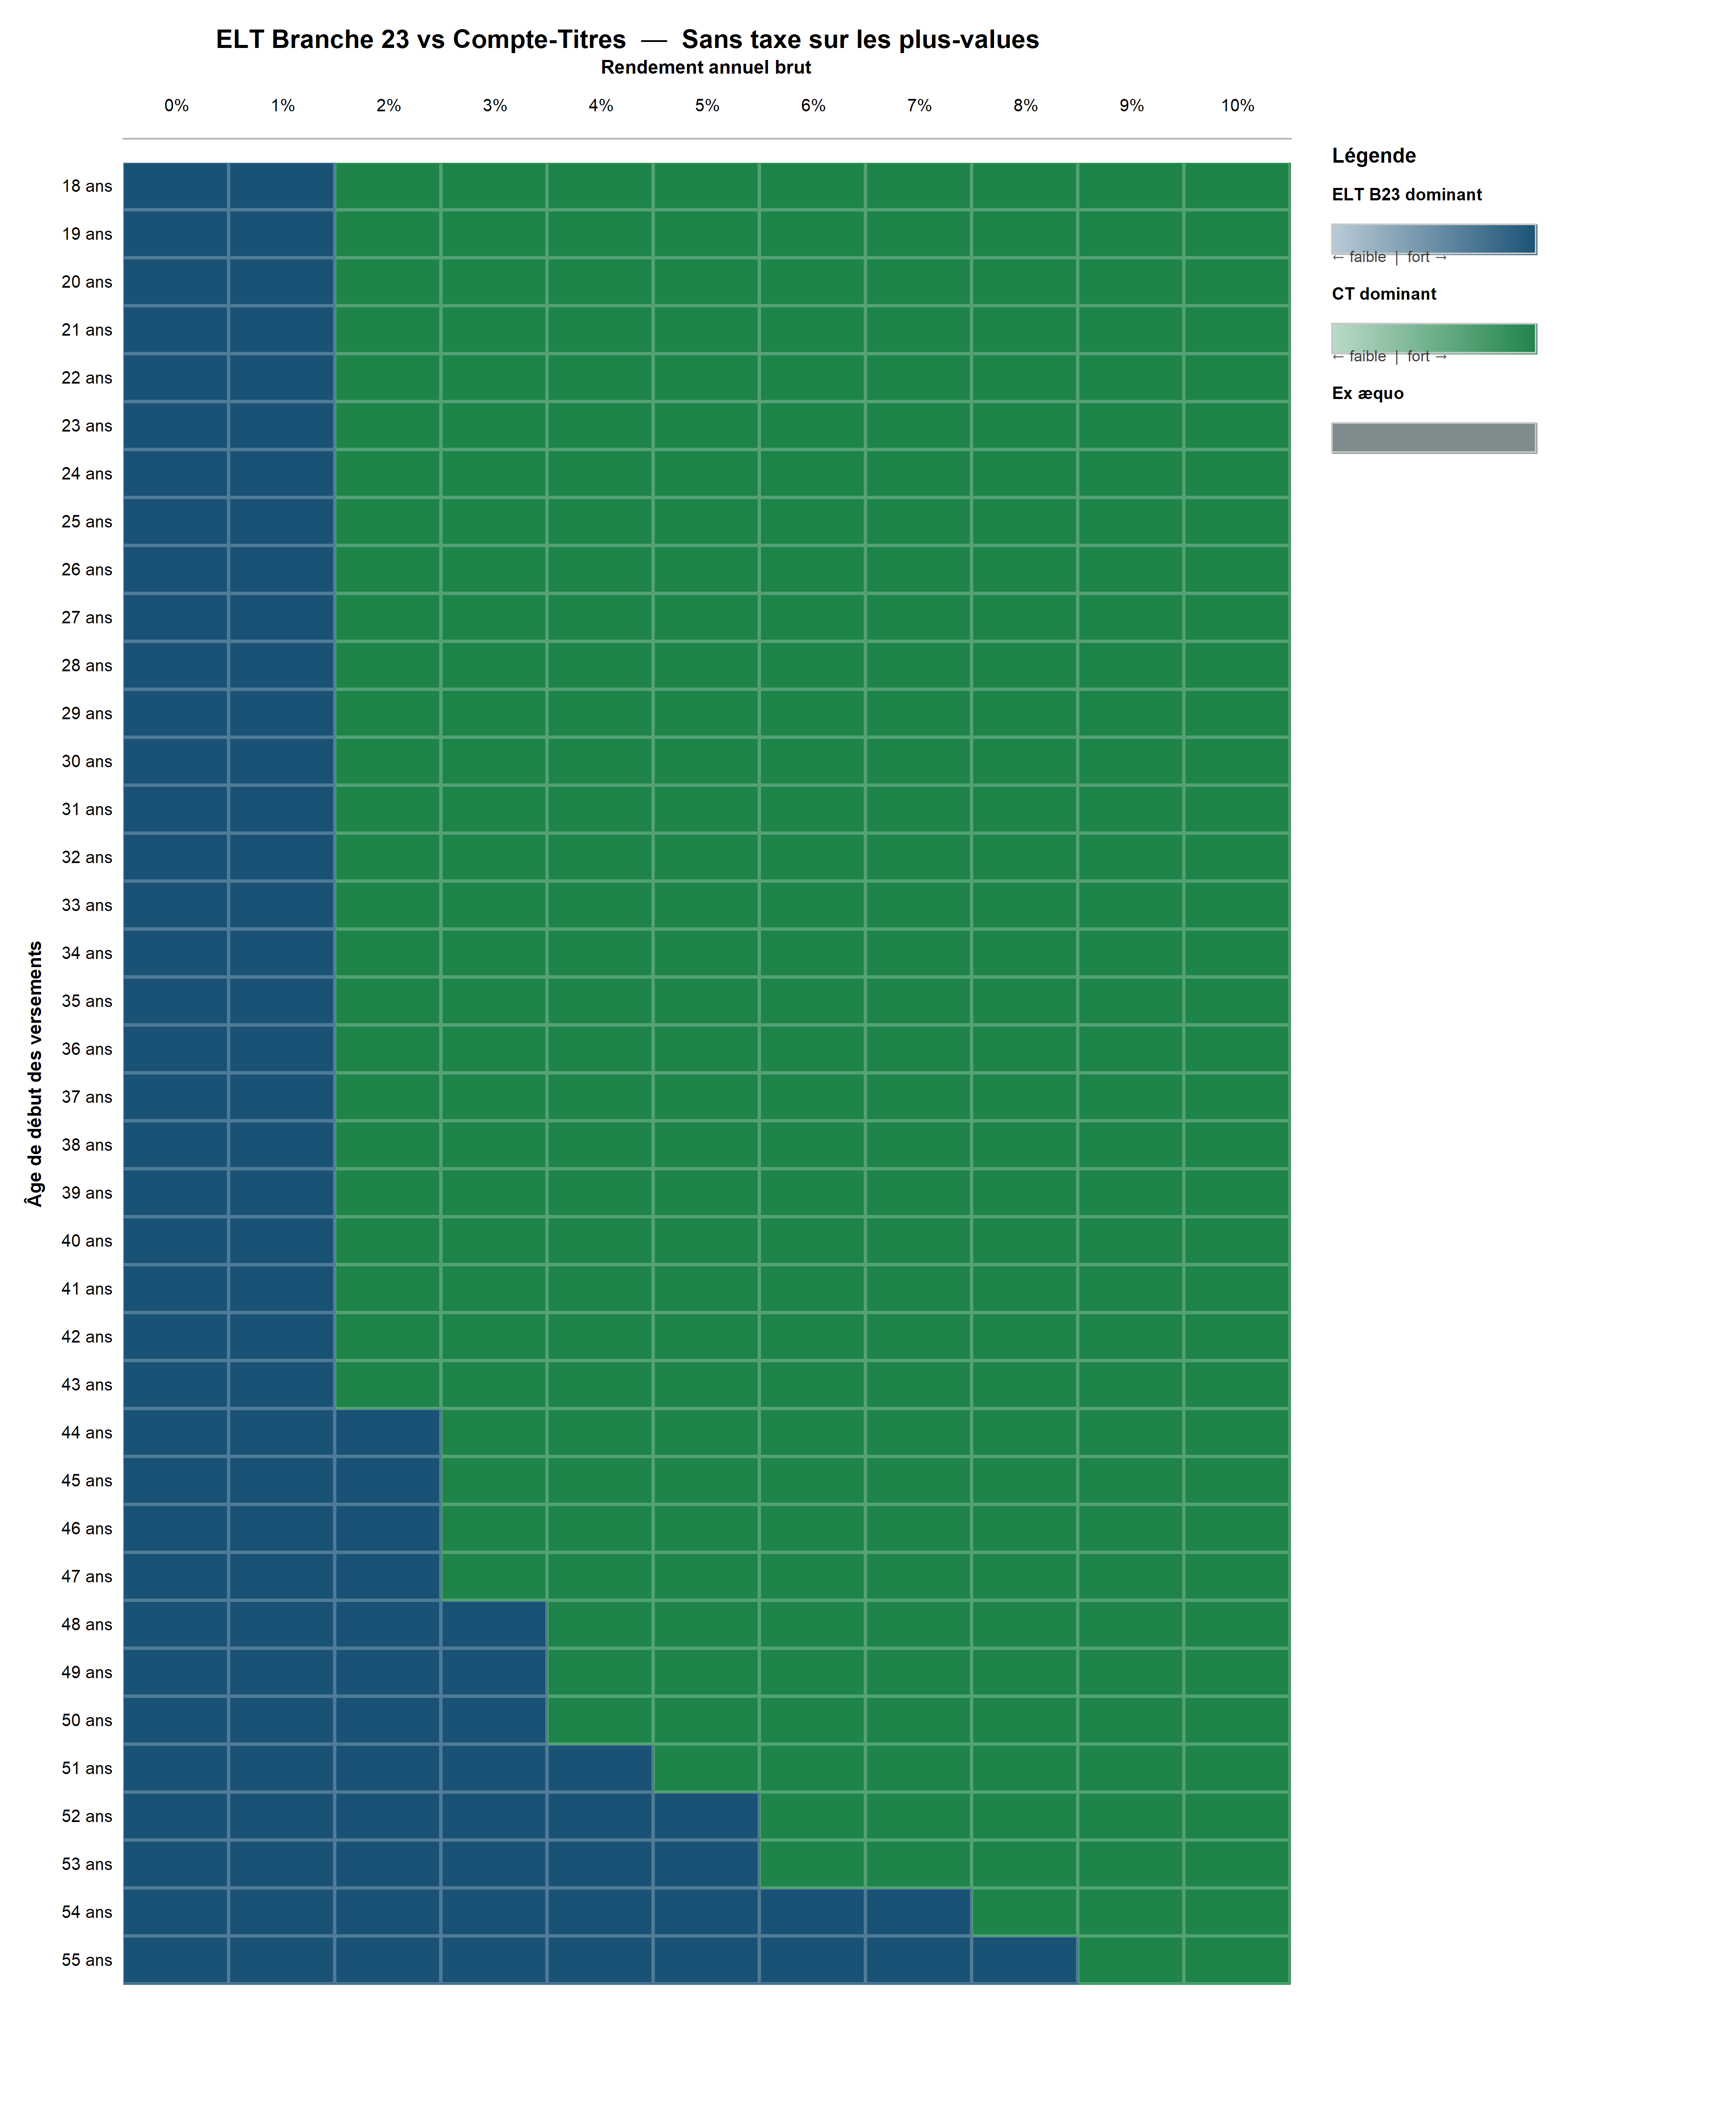
\includegraphics[width=\textwidth]{media/elt_frais_reel_sans_taxe.png}
  \caption{Dominance ELT\,/\,CT --- Scénario~B (frais réalistes), sans taxe sur les plus-values.}
  \label{fig:ann_elt_frais_reel_sans_taxe}
\end{figure}

\begin{figure}[H]
  \centering
  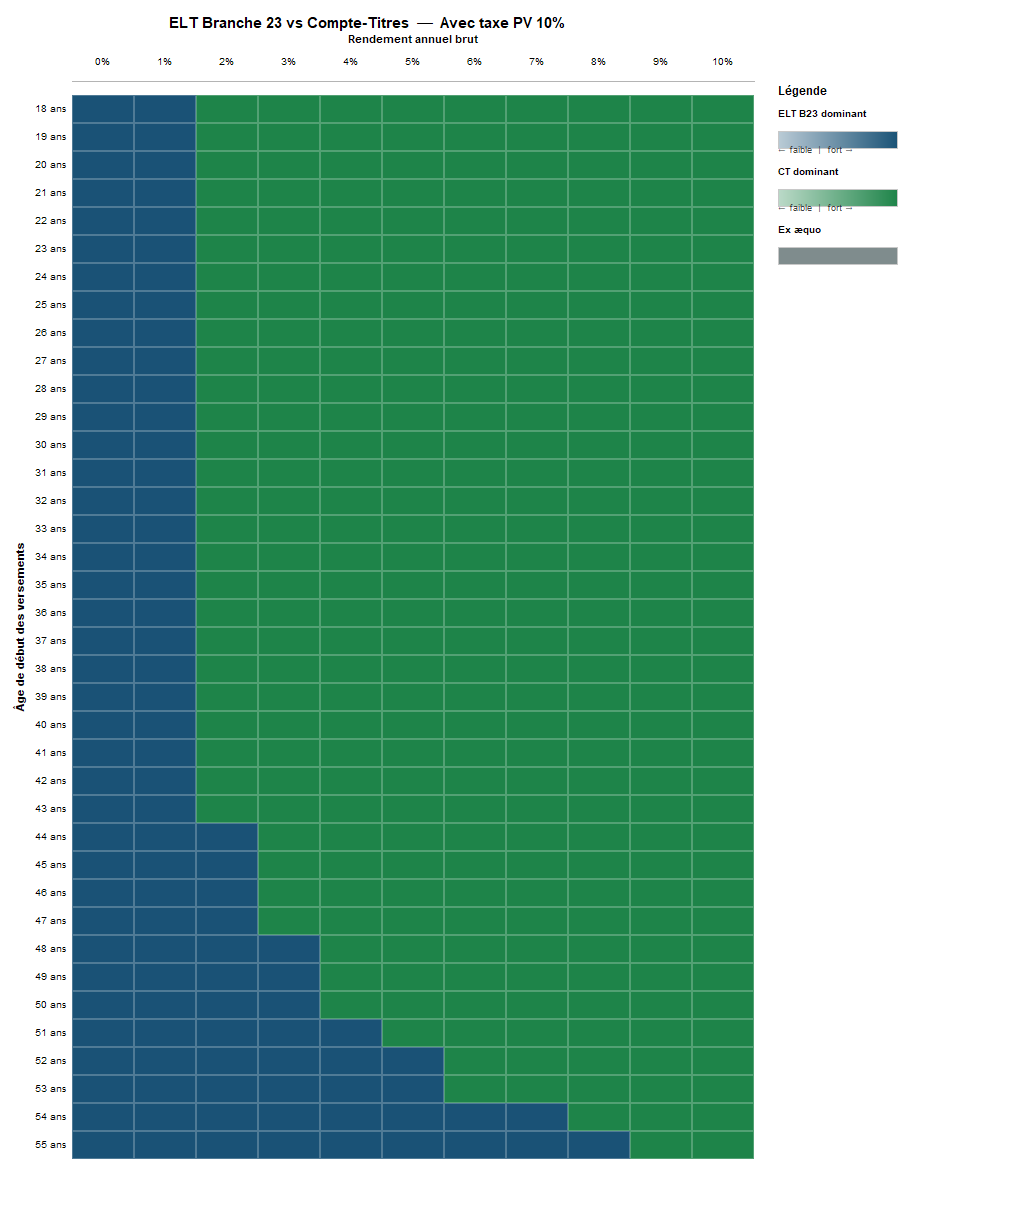
\includegraphics[width=\textwidth]{media/elt_frais_reel_avec_taxe.png}
  \caption{Dominance ELT\,/\,CT --- Scénario~B (frais réalistes), avec taxe sur les plus-values de 10\,\%.}
  \label{fig:ann_elt_frais_reel_avec_taxe}
\end{figure}

%==========================================================================
\section{Heatmaps ELT\,/\,CT --- Scénario~C (frais majorés)}
\label{ann:heatmaps_C}

\begin{figure}[H]
  \centering
  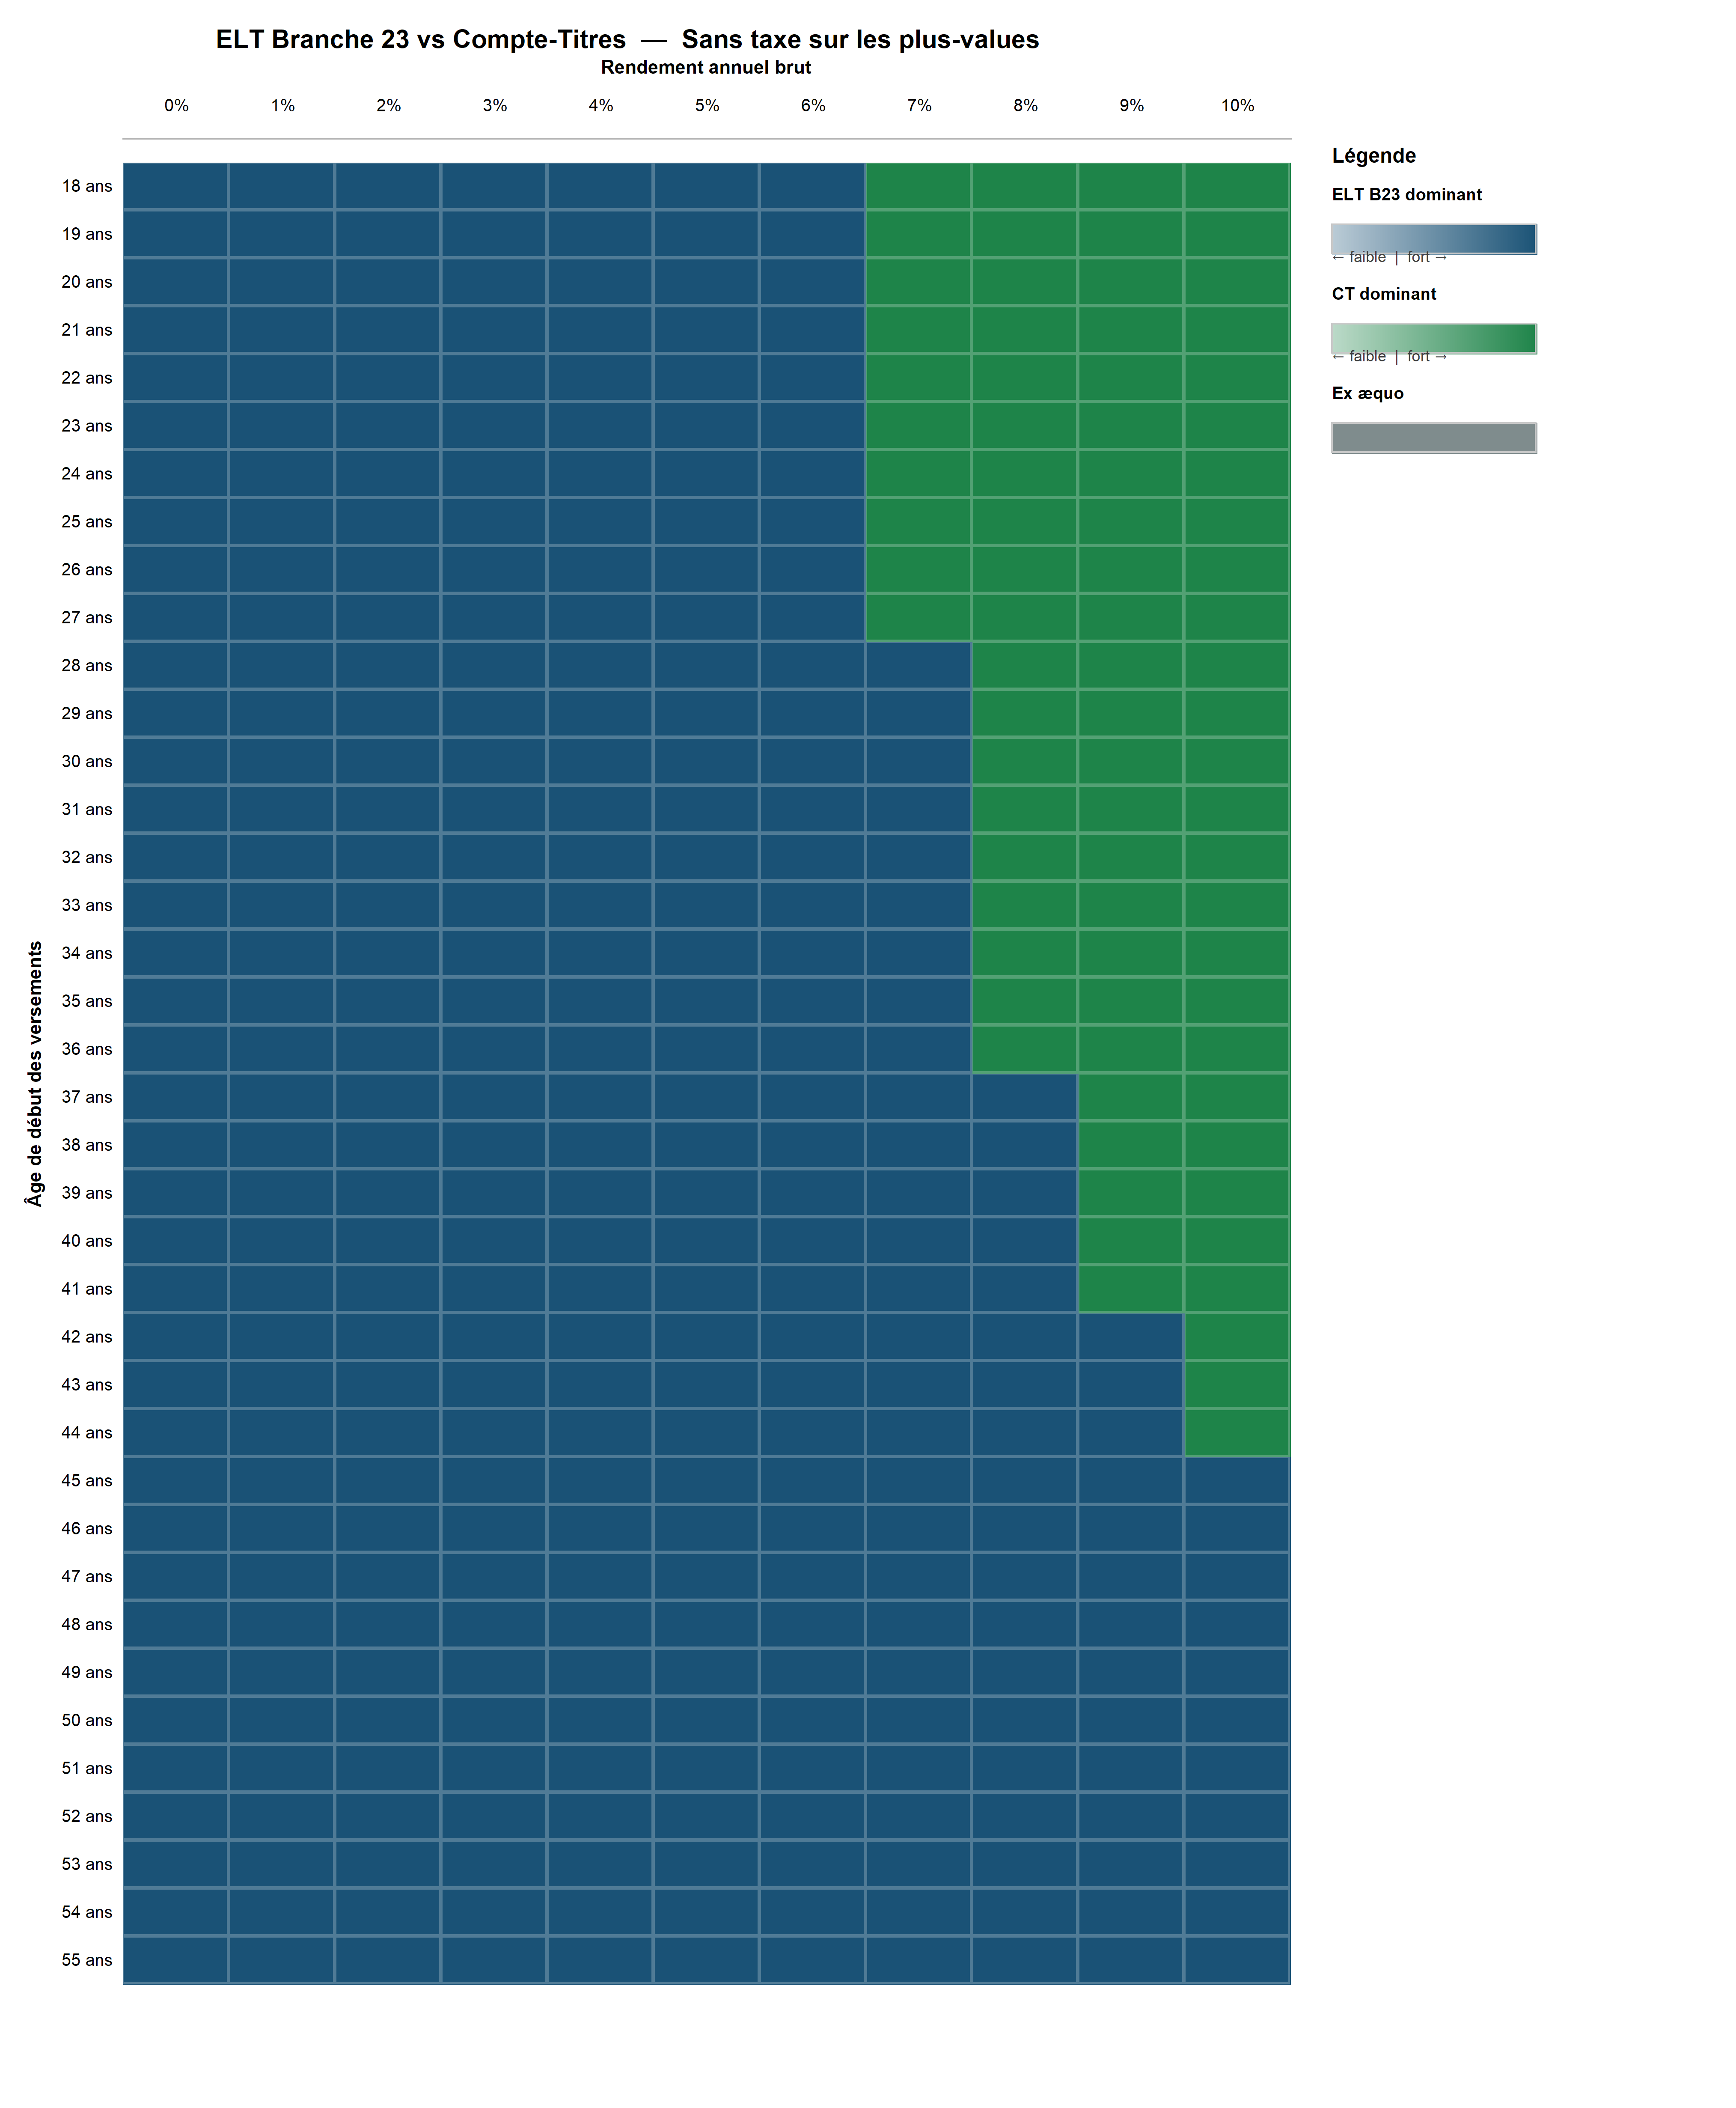
\includegraphics[width=\textwidth]{media/elt_frais_majore_sans_taxe.png}
  \caption{Dominance ELT\,/\,CT --- Scénario~C (frais égalisés), sans taxe sur les plus-values.}
  \label{fig:elt_frais_majore_sans_taxe}
\end{figure}

\begin{figure}[H]
  \centering
  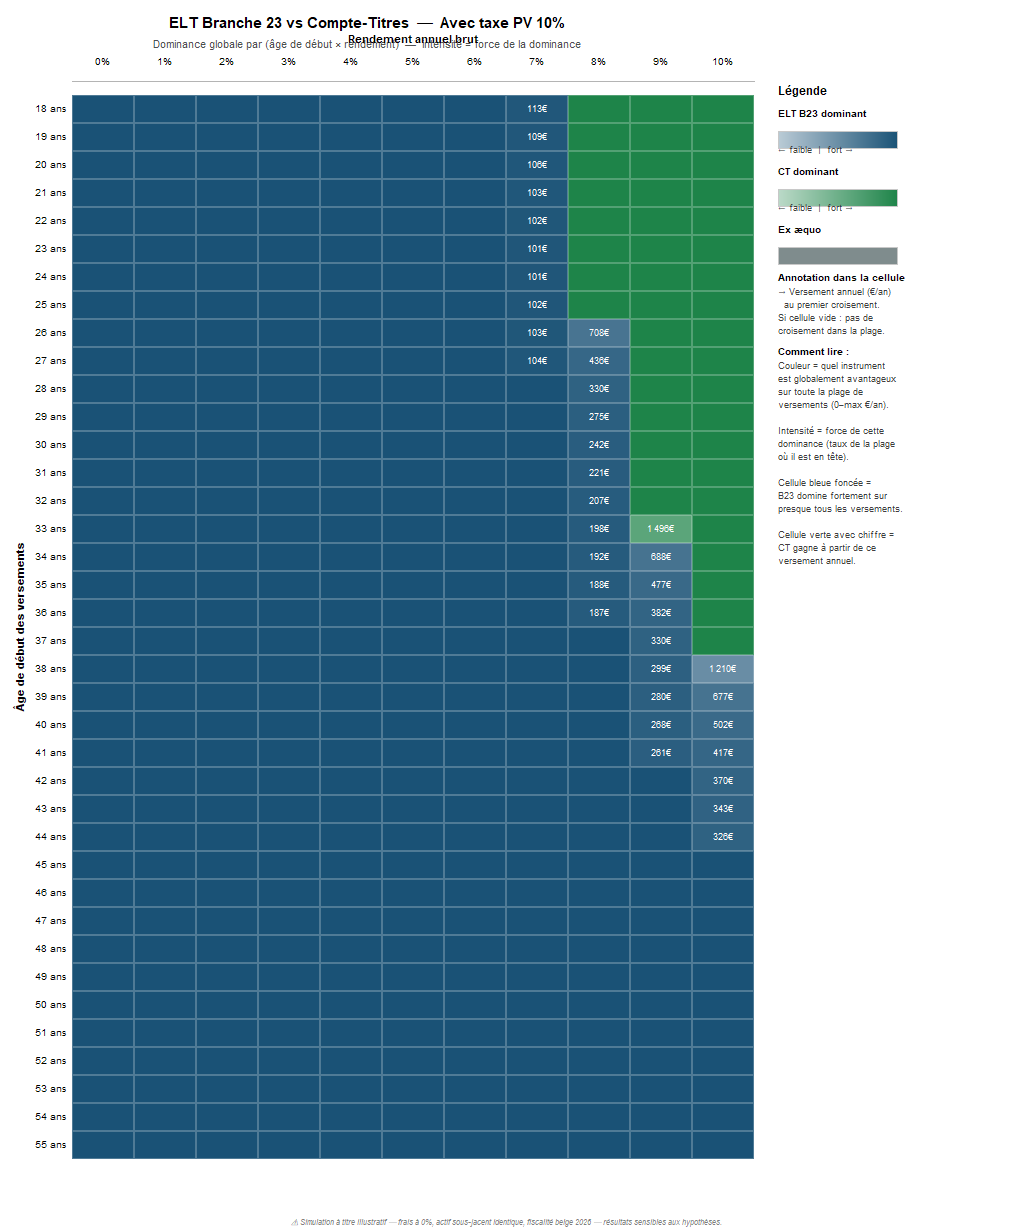
\includegraphics[width=\textwidth]{media/elt_frais_majore_avec_taxe.png}
  \caption{Dominance ELT\,/\,CT --- Scénario~C (frais égalisés), avec taxe sur les plus-values de 10\,\%.}
  \label{fig:elt_frais_majore_avec_taxe}
\end{figure}

%==========================================================================
\section{Heatmaps EP\,/\,CT --- Scénario~A (effet fiscal pur)}
\label{ann:heatmaps_ep_A}

\begin{figure}[H]
  \centering
  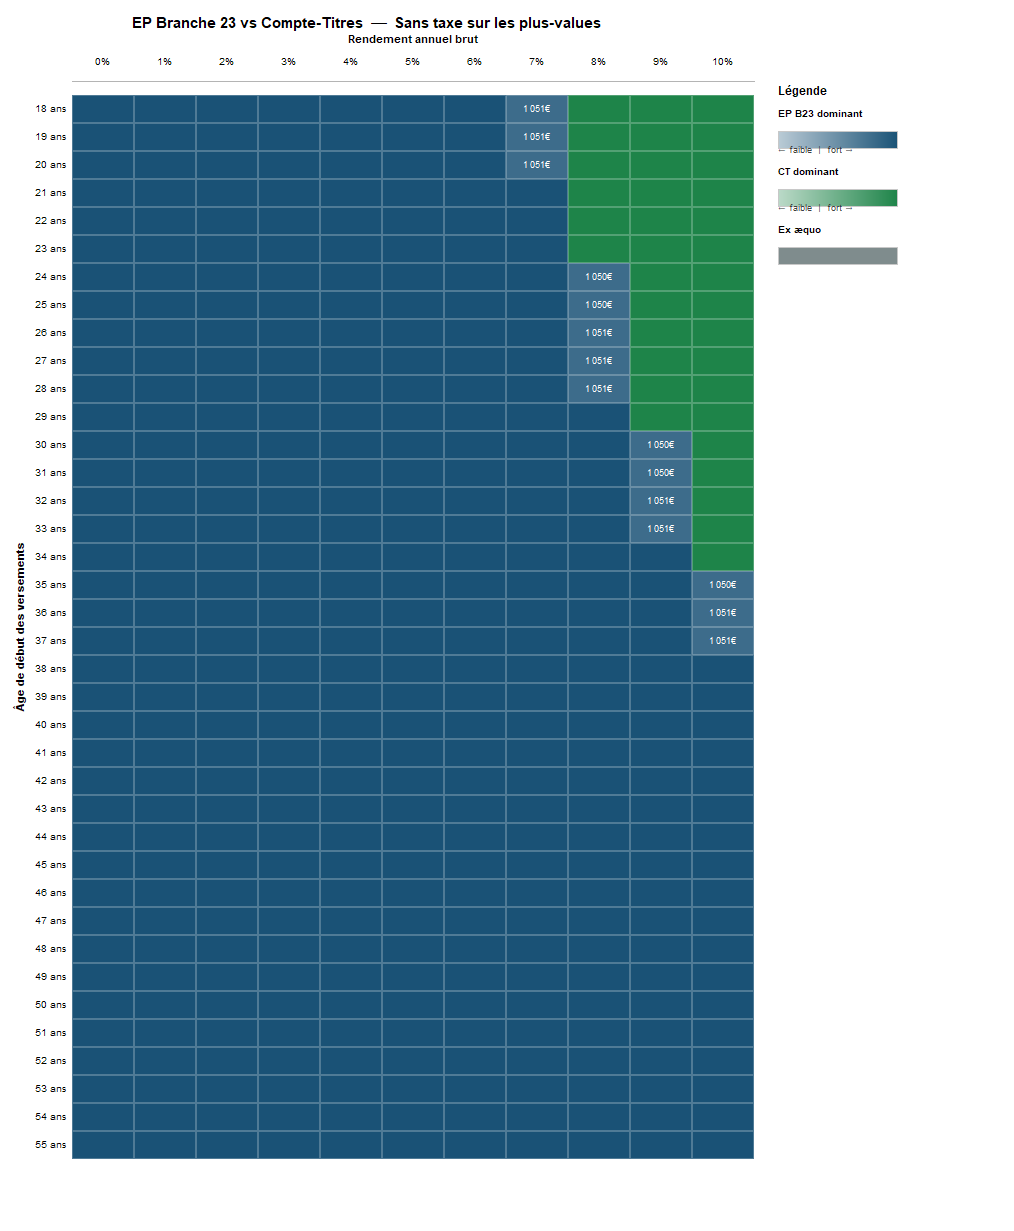
\includegraphics[width=\textwidth]{media/ep_frais_0_sans_taxe.png}
  \caption{Dominance EP\,/\,CT --- Scénario~A (aucun frais), sans taxe sur les plus-values.}
  \label{fig:ep_frais_0_sans_taxe}
\end{figure}

\begin{figure}[H]
  \centering
  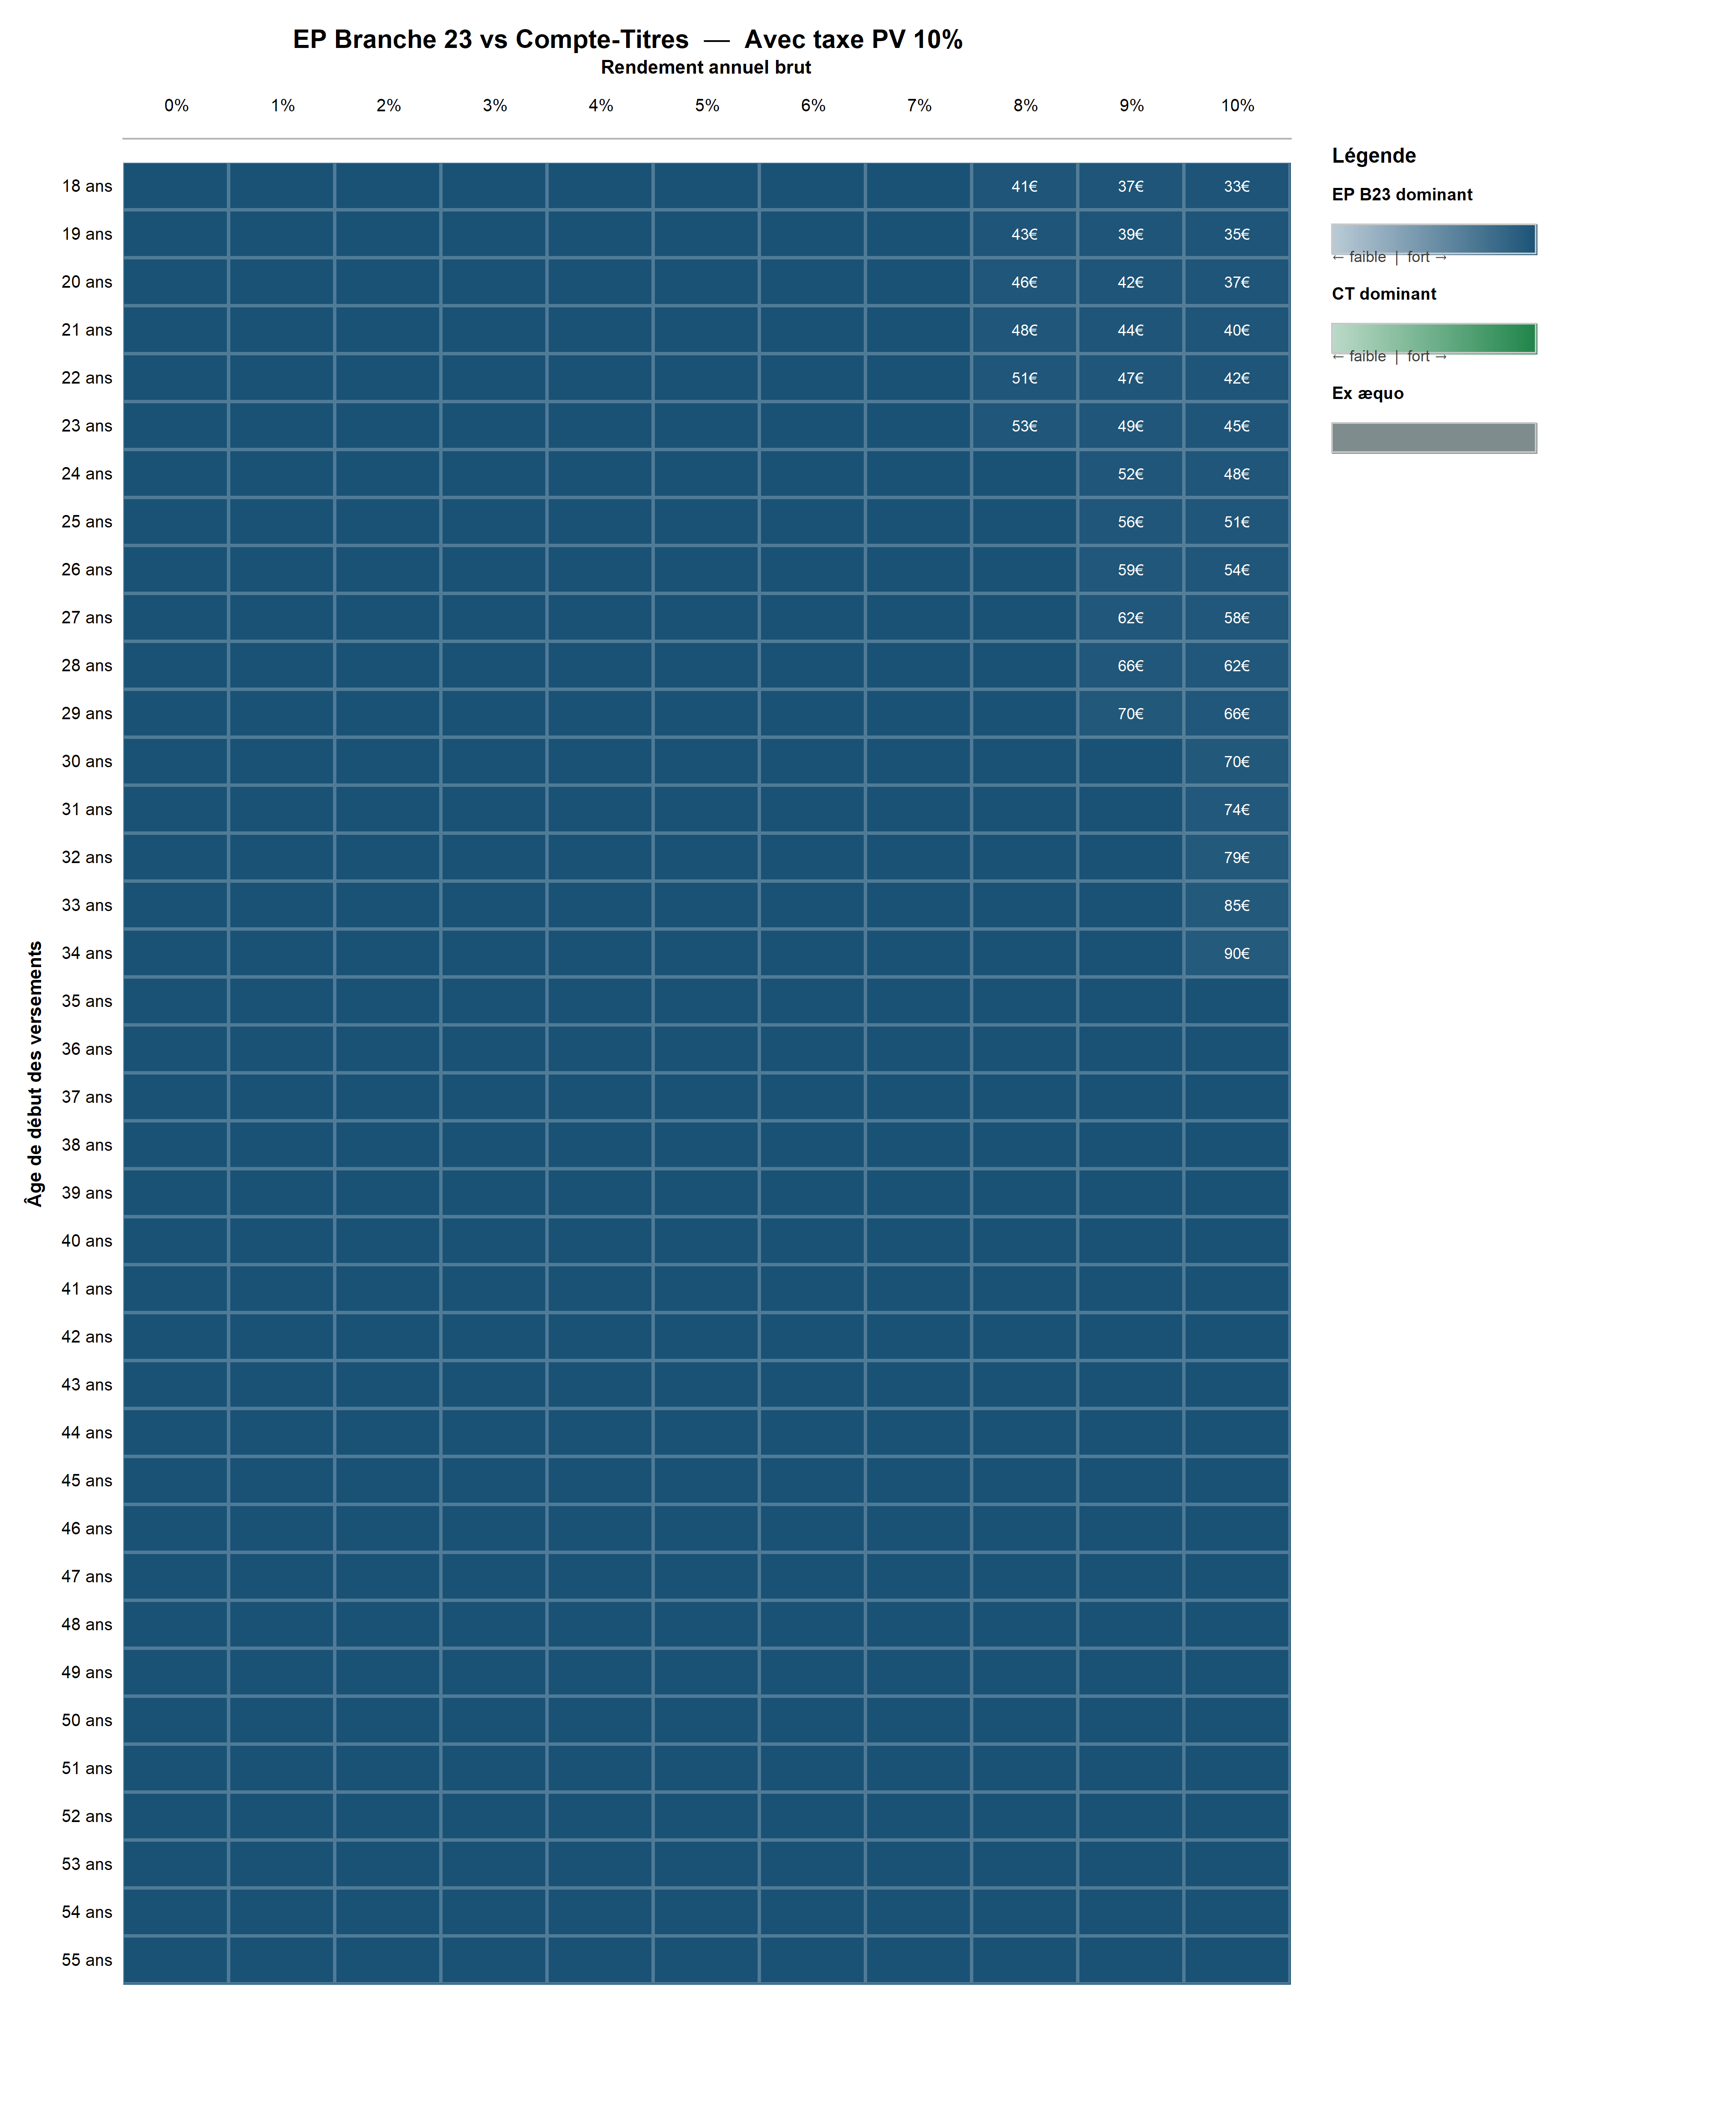
\includegraphics[width=\textwidth]{media/ep_frais_0_avec_taxe.png}
  \caption{Dominance EP\,/\,CT --- Scénario~A (aucun frais), avec taxe sur les plus-values de 10\,\%.}
  \label{fig:ep_frais_0_avec_taxe}
\end{figure}

%==========================================================================
\section{Heatmaps EP\,/\,CT --- Scénario~B (frais réalistes)}
\label{ann:heatmaps_ep_B}

\begin{figure}[H]
  \centering
  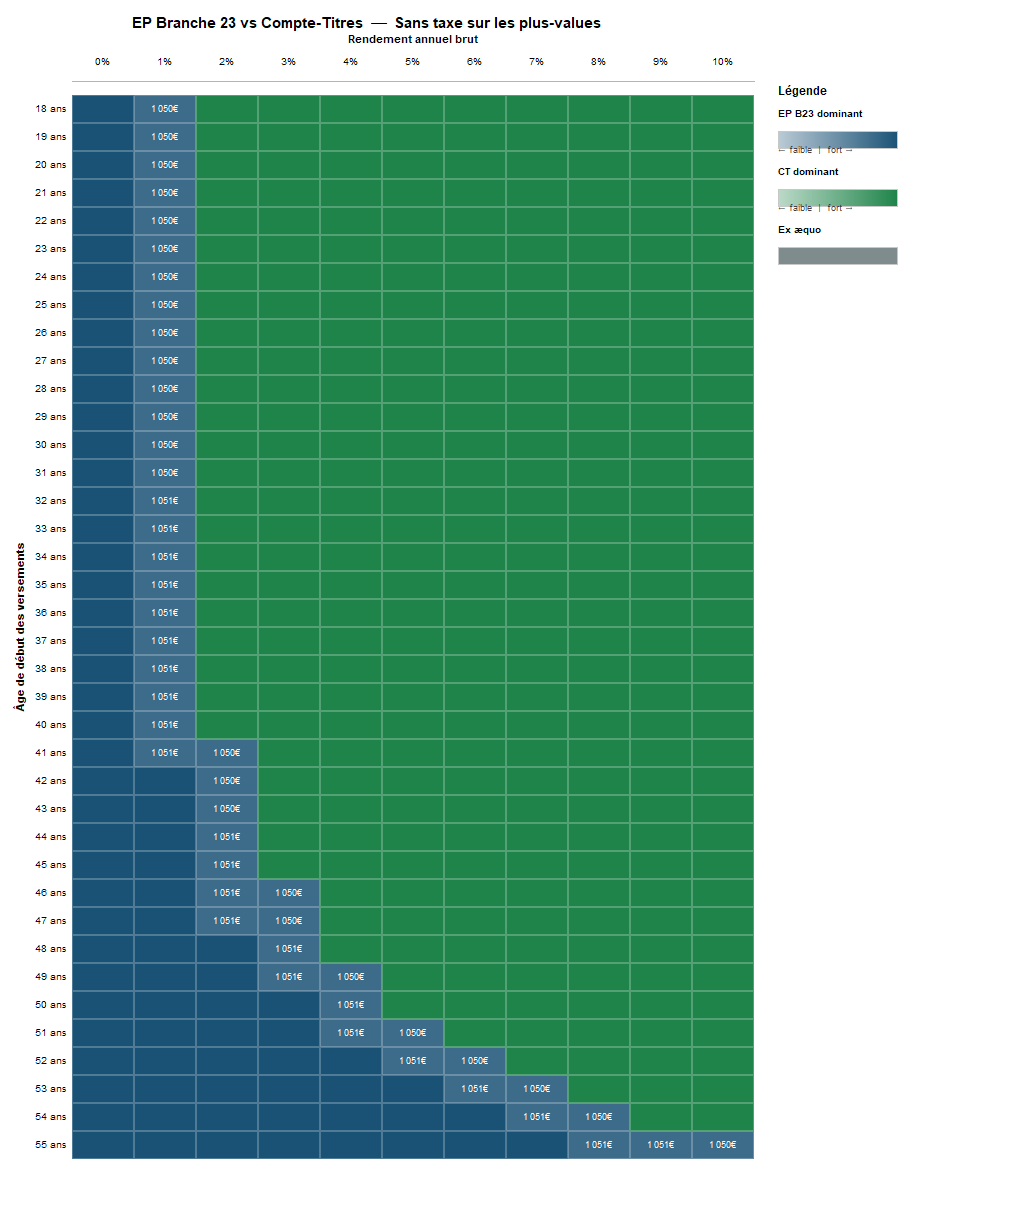
\includegraphics[width=\textwidth]{media/ep_frais_reel_sans_taxe.png}
  \caption{Dominance EP\,/\,CT --- Scénario~B (frais réalistes), sans taxe sur les plus-values.}
  \label{fig:ann_ep_frais_reel_sans_taxe}
\end{figure}

\begin{figure}[H]
  \centering
  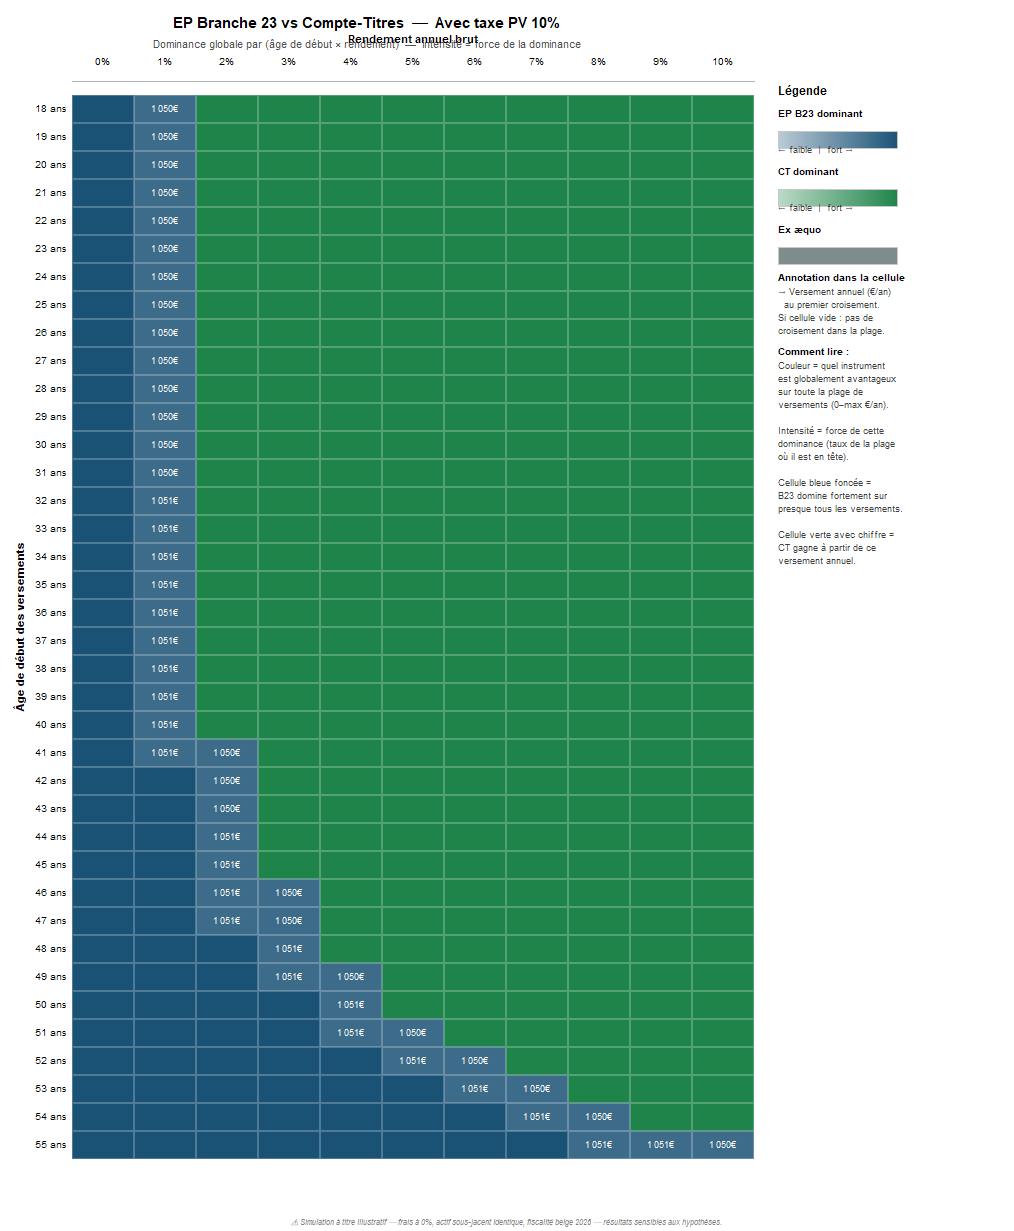
\includegraphics[width=\textwidth]{media/ep_frais_reel_avec_taxe.png}
  \caption{Dominance EP\,/\,CT --- Scénario~B (frais réalistes), avec taxe sur les plus-values de 10\,\%.}
  \label{fig:ann_ep_frais_reel_avec_taxe}
\end{figure}

%==========================================================================
\section{Heatmaps EP\,/\,CT --- Scénario~C (frais majorés)}
\label{ann:heatmaps_ep_C}

\begin{figure}[H]
  \centering
  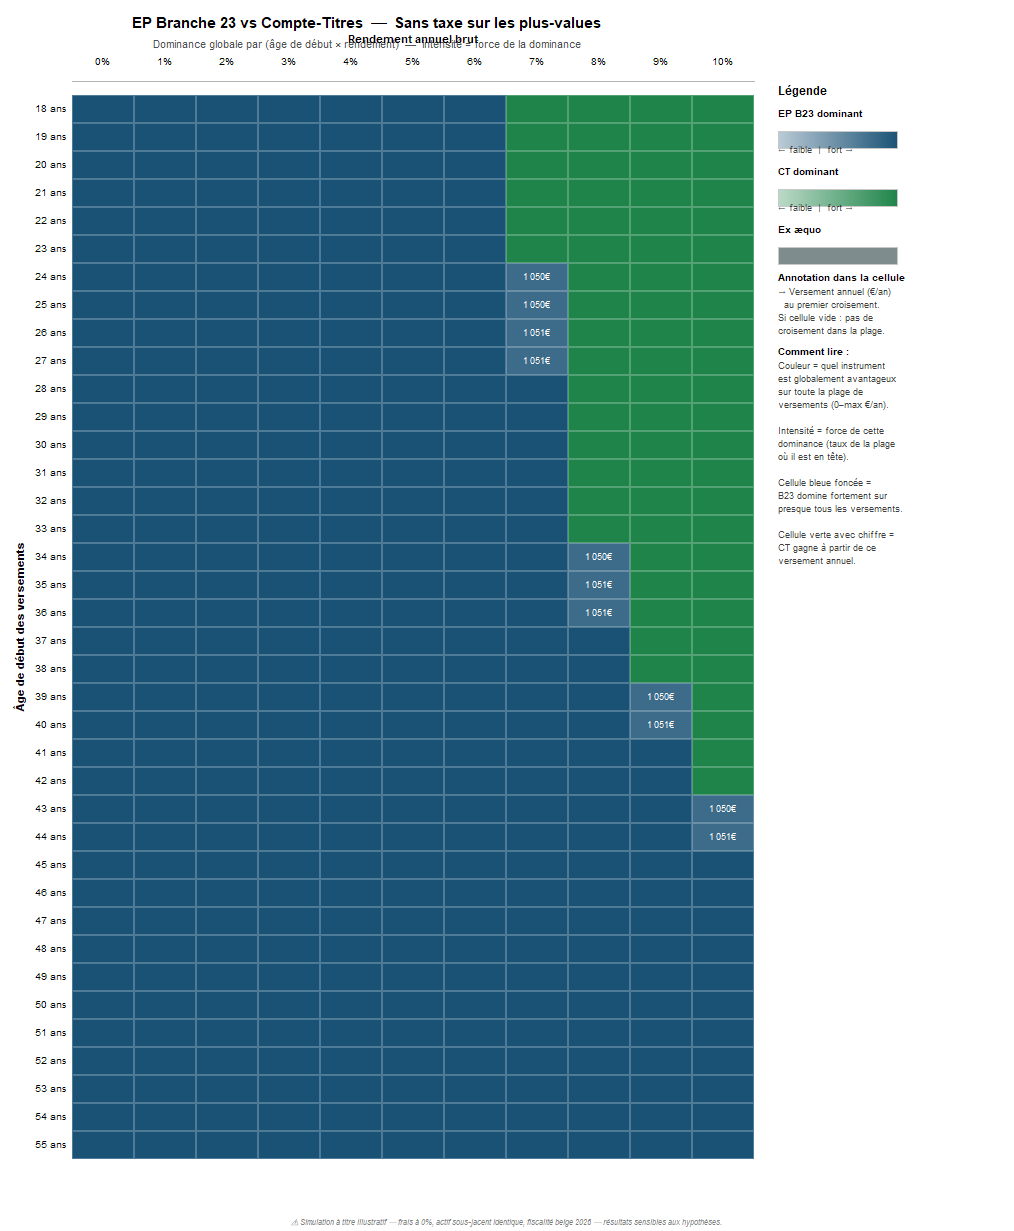
\includegraphics[width=\textwidth]{media/ep_frais_majore_sans_taxe.png}
  \caption{Dominance EP\,/\,CT --- Scénario~C (frais égalisés), sans taxe sur les plus-values.}
  \label{fig:ep_frais_majore_sans_taxe}
\end{figure}

\begin{figure}[H]
  \centering
  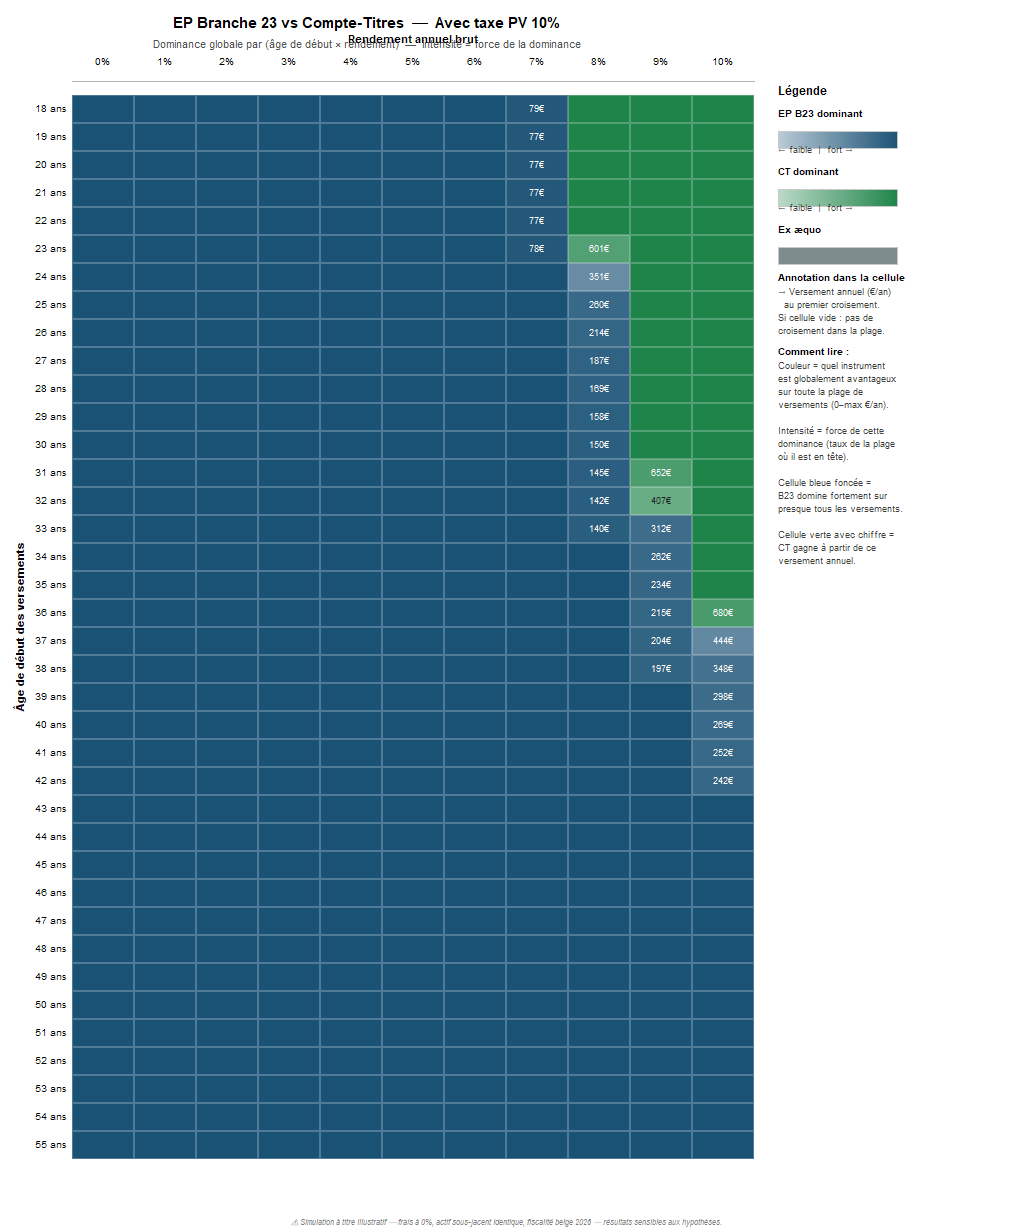
\includegraphics[width=\textwidth]{media/ep_frais_majore_avec_taxe.png}
  \caption{Dominance EP\,/\,CT --- Scénario~C (frais égalisés), avec taxe sur les plus-values de 10\,\%.}
  \label{fig:ep_frais_majore_avec_taxe}
\end{figure}

%==========================================================================
\section{Structure des fichiers de données produits par la simulation}
\label{ann:csv_colonnes}

La simulation produit quatre fichiers de données structurés (format CSV), un
par scénario de comparaison. Chaque fichier contient une ligne par combinaison
(âge de début~$\times$~rendement annuel). Le tableau ci-dessous décrit les
colonnes présentes dans chacun de ces fichiers.

\begin{table}[h!]
  \centering
  \caption{Description des colonnes des fichiers de données de simulation}
  \label{tab:csv_colonnes}
  \small
  \begin{tabular}{lp{9cm}}
    \hline
    \textbf{Colonne} & \textbf{Description} \\
    \hline
    \texttt{vehicule\_a} & Nom du véhicule A (ex.~«~EP Branche~23~») \\
    \texttt{vehicule\_b} & Nom du véhicule B (ex.~«~CT taxe PV 10\,\%~») \\
    \texttt{rendement\_pct} & Rendement annuel brut simulé (en \%) \\
    \texttt{age\_debut} & Âge de début des versements \\
    \texttt{age\_fin} & Âge de fin de l'horizon (65~ans) \\
    \texttt{taux\_taxe\_pv\_pct} & Taux de la taxe sur les plus-values appliqué au CT (0 ou 10) \\
    \texttt{versement\_min} & Borne inférieure de la plage de versements (1~€) \\
    \texttt{versement\_max} & Borne supérieure de la plage (1\,350~€ ou 2\,450~€) \\
    \texttt{taux\_dominance\_A\_pct} & Part des versements (en \%) pour lesquels la valeur terminale de~A dépasse celle de~B \\
    \texttt{taux\_dominance\_B\_pct} & Part des versements (en \%) pour lesquels la valeur terminale de~B dépasse celle de~A \\
    \texttt{taux\_egaux\_pct} & Part des versements (en \%) pour lesquels les deux valeurs terminales sont égales \\
    \texttt{nb\_croisements} & Nombre de points de croisement détectés sur la plage \\
    \texttt{premier\_croisement\_eur} & Montant du versement au premier croisement (en~€, ou \texttt{NA} si absent) \\
    \texttt{dominant} & Véhicule globalement dominant sur la plage (chaîne descriptive) \\
    \texttt{capital\_final\_net\_moyen\_b23\_eur} & Capital net moyen du véhicule~A sur la plage de versements (en~€) \\
    \texttt{eco\_fiscales\_capitalisees\_moyennes\_b23\_eur} & Économies fiscales annuelles capitalisées à l'échéance, en moyenne sur la plage (en~€) \\
    \texttt{val\_terminale\_moyenne\_ct\_eur} & Valeur terminale nette moyenne du CT sur la plage de versements (en~€) \\
    \hline
  \end{tabular}
\end{table}

\end{document}
